\documentclass[12pt,oneside,a4paper]{abntex2}                 

%\usepackage[brazil]{babel}
%citaçoes
%\usepackage[alf]{abntcite} 

\usepackage{cmap} 
\usepackage{lmodern}                    
\usepackage[usenames,dvipsnames]{pstricks}
\usepackage{graphicx}
\usepackage{epstopdf}
\usepackage{enumerate}
\usepackage{amsmath,bm}
\usepackage[framed, numbered]{matlab-prettifier}
\usepackage{float}
\usepackage{multicol}
\usepackage{mathptmx}
\usepackage{esvect}
\usepackage{amssymb,indentfirst}  
\usepackage[T1]{fontenc}        
\usepackage[utf8]{inputenc}          
\usepackage{makeidx}         
\usepackage{hyperref}           
\usepackage{lastpage}                   
\usepackage{indentfirst}              
\usepackage{nomencl}           
\usepackage{color}                             
\usepackage{graphicx}             
\usepackage{pdfpages}


\hyphenation{Magneto-hydro-dynamics}
\hyphenation{ele-tro-mag-né-ti-cas}
\hyphenation{nu-me-ri-ca-men-te}
\hyphenation{mag-né-ti-co}
\hyphenation{mag-né-ti-cos}
\hyphenation{con-tri-bui-ção}
\hyphenation{nu-mé-ri-ca}
\hyphenation{atra-vés}
\hyphenation{con-ser-va-ção}
\hyphenation{co-or-de-na-das}
\hyphenation{equa-cio-na-men-to}
\hyphenation{break-down}
\hyphenation{di-re-ta-men-te}
\hyphenation{mul-ti-pli-can-do}
\hyphenation{pseudo-to-roi-dais}
\hyphenation{ele-tro-mag-né-ti-ca}
\hyphenation{pro-prie-da-des}
\hyphenation{tri-di-men-sio-nal}
\hyphenation{su-fi-ci-en-te-men-te}
\hyphenation{coe-fi-ci-en-tes}
\hyphenation{pre-do-mi-nan-te-men-te}
\hyphenation{im-ple-men-ta-ção}
\hyphenation{fi-si-ca-men-te}
\hyphenation{di-fe-ren-ciais}
\hyphenation{par-tí-cu-las}
\hyphenation{co-li-sio-na-is}
\hyphenation{ele-tro-mo-triz}
\hyphenation{con-cer-va-ção}
\hyphenation{ma-cros-có-pi-cas}
\hyphenation{per-mi-ssi-vi-da-de}
\hyphenation{cor-res-pon-den-te}
\hyphenation{pro-gres-si-vas}
\hyphenation{mo-de-lan-do}
\hyphenation{pro-ces-sa-men-to}
\hyphenation{aque-ci-men-to}
\hyphenation{com-por-ta-men-to}
\usepackage[normalem]{ulem}    
% ---
 \definecolor{lightblue}{rgb}{0.68,0.85,0.9}
 \definecolor{indianred}{rgb}{0.8,0.36,0.36}


\titulo{{Estudos de breakdown no tokamak TCABR-USP}}
\autor{Kévi Pegoraro}
\local{Rio Grande, Rio Grande do Sul, Brasil}
\data{\today}
\orientador{{--}}
\coorientador{{Dr. Gustavo P. Canal}}
\instituicao{%
  Universidade Federal do Rio Grande - FURG
  \par
  Instituto de Matemática, Estatística e Física - IMEF
  \par
  Curso de Mestrado em modelagem computacional}
\tipotrabalho{Tese para conclusão de curso}
\preambulo{Tese para conclusão de curso, Mestrado em modelagem computacional. Universidade Federal do Rio Grande.}
\definecolor{blue}{RGB}{41,5,195}

%\newcommand{\nablab}{\textit{\boldsymbol{\nabla}}}

\setlength{\parindent}{1.3cm}

\setlength{\parskip}{0.2cm}  % tente também 

\makeindex

\makenomenclature
\begin{document}
%\maketitle
%\UseRawInputEncoding
%\date[2019]{\today}

\imprimircapa
\imprimirfolhaderosto
\cleardoublepage


%\begin{agradecimentos}
%\noindent Ao Dr. Magno Pinto Collares (FURG) e ao Dr. Gustavo Paganini Canal (USP) por terem aceitado me orientar, por ensinarem, instruírem e colaborarem tanto para minha formação científica e pessoal. Agradeço também pela ajuda com materiais de estudo, respostas a inúmeras dúvidas e ajuda no desenvolvimento da fase teórica e computacional. 

%\noindent Ao Dr. Igor Oliveira Monteiro (FURG) pela ajuda com dúvidas na parte numérica.  

%\noindent Aos membros da banca por terem aceitado ler e corrigir meu trabalho.

   %\vspace*{\fill}
   %\centering
   %\noindent
  % \textit{\\ Este trabalho é dedicado à minha esposa Taionara Silva da Silva.}
   
 %  \vspace{.3cm}
%\end{agradecimentos}
%PAGINAS DE INTRODUÇAO
%\tableofcontents
%\newpage
%\listoffigures
%\newpage
%\listoftables
%\newpage
%\lstlistoflistings
%\bibliographystyle{plain}
%\newpage
%\mainmatter
\chapter*{Lista de notações}
\label{Listanot}
\noindent Na lista de notações, $X_\alpha$ com o índice $\alpha$ denota a propriedade $X$ para as partículas da espécie $\alpha$:\\
\begin{itemize}
\item $\phi$ é o ângulo na direção toroidal; 
\item $r$ é a coordenada radial na direção poloidal;  
\item $z$ é a coordenada vertical na direção poloidal;
\item $f_\alpha(\bm{r},\bm{v},t)$ é a função distribuição de velocidades;
\item $\bm{F}_{ext}$ é a força externa, incluindo a força de Lorentz associada a quaisquer campos elétricos e magnéticos aplicados externamente;
\item $\mu_0$ é a permeabilidade magnética do vácuo;
\item $c$ é a velocidade da luz no vácuo; 
\item $\epsilon_0$ é constante de permissividade do vácuo; % = \frac{1}{\mu_0 c^2}
\item $k_B$ é a constante de Boltzmann;
\item $\bm{A}_{pl}$ é o vetor potencial magnético devido ao plasma;
\item $R_0$ é o raio externo da câmera de vácuo;
\item $V_{loop}$ é a voltagem de \textit{loop} toroidal induzida pelo solenoide central;
\item $B_0$ é a intensidade inicial do campo magnético toroidal; 
\item $a_0$ é o raio interno da câmera de vácuo;
%\item $\bm{E}_{pl}$ é o vetor campo elétrico macroscópico interno; %unidade N/C;
%\item $\bm{B}_{pl}$ é o vetor campo magnético macroscópico interno;
\item $S_\alpha$ é o termo de fonte de partículas;
\item $\bm{B}_{pl}$ é o vetor campo magnético gerado pelo plasma; % unidade T;
\item $\bm{E}_{pl}$ é o vetor campo elétrico gerado pelo plasma;
\item $\bm{B}_{ext}$ é o vetor campo magnético externo;
\item $\bm{E}_{ext}$ é o vetor campo elétrico externo;
\item $\bm{B}$ é o vetor campo magnético total;%= \bm{B}_{ext} + \bm{B}_{pl}$
\item $\bm{E}$ é o vetor campo elétrico total; %= \bm{E}_{ext} + \bm{E}_{pl}
\item $n_{\alpha}(\bm{r},t)$ é a densidade de plasma ou densidade numérica de partículas; %= \int{f_\alpha(\bm{r},\bm{v},t)}d\bm{v}
\item $n_i(\bm{r},t)$ é a densidade numérica de íons;
\item $n_e(\bm{r},t)$ é a densidade numérica de elétrons;
\item $n_g$ é a densidade inicial de partículas neutras;
\item $\bm{J}(\bm{r},t)$ é vetor densidade de corrente; %unidade A;
\item $p_\alpha(\bm{r},t)$ é o escalar de pressão;
\item $T_{\alpha 0}$ é a temperatura inicial; % unidade 
%\item $T_{e}$ é a temperatura de elétrons;
%\item $T_{e,i}$ é a temperatura de elétrons e íons;
\item $\nu_{en}$ é a taxa de ionização elétron-nêutrons; % unidade 1/s;
\item $\nu_{in}$ é a taxa de ionização íon-nêutrons;
\item $\nu_{ei}$ é a taxa de ionização elétron-íon;
\item $\nu_{loss}$ é a taxa de perda de elétrons;
\item $\nu_{eff}$ é a frequência efetiva de colisão de elétrons;%=\nu_{ei} + \nu_{en} + \nu_{in} + \nu_{loss}
\item $\bm{u}_{\alpha}(\bm{r},t)$ é o vetor velocidade média das partículas; %em $v = \frac{1}{n(\bm{r},t)} \int_V{\bm{v} f_{\alpha}(\bm{r},\bm{v},t) d^3v}
\item $m_\alpha$ é a massa do tipo de partícula $\alpha$; %unidade Kg;
\item $\alpha_a$ é o primeiro coeficiente de Townsend;
\item $\tau_p$ é o tempo médio de confinamento da partícula;
\item $\rho_\alpha(\bm{r},t)$ é a densidade de carga;
\item $\rho_{m\alpha}(\bm{r},t)$ é a densidade de massa;
\item $M_\alpha$ é a taxa de variação da densidade de energia devido à produção e aniquilação de partículas;
\item $Q_\alpha$ é a taxa de mudança de densidade de energia devido ao espalhamento;
\item $\mathcal{E}_\alpha$ é a produção de partículas de plasma;
\item $\mathbb{P}_\alpha$ é o tensor de pressão cinética; %= \rho_{m\alpha}<\bm{c} \cdot \bm{c}>_\alpha
\item $\bm{q}_\alpha $ é o vetor fluxo de calor; %= \frac{1}{2} \rho_{m\alpha} <c^2_\alpha  \bm{c}_\alpha>
\item $q_\alpha$ é carga da partícula;
\item $D_\alpha$ é o coeficientes de difusão de partículas;
\item $e$ é a carga elementar do elétron;
\item $\eta$ é a resistividade paralela do Spitzer;
\item $\bm{R}_\alpha$ é o vetor de troca de momento;
\item $\bm{R}_\alpha$ é a taxa de mudança de momento devido ao espalhamento e a taxa de mudança de momento devido à produção de partículas de plasma.


\end{itemize}

\section*{Operadores diferenciais}
\subsection*{Cartesianas}
\begin{equation}
\bm{\nabla} = \hat{e}_x \frac{\partial}{\partial x} + \hat{e}_y \frac{\partial}{\partial y} + \hat{e}_z \frac{\partial}{\partial z},
\end{equation}
\begin{equation}
\nabla^2 =  \frac{\partial^2}{\partial x^2} +  \frac{\partial^2}{\partial y^2} + \frac{\partial^2}{\partial z^2},
\end{equation} %\hat{e}_x  \hat{e}_z \hat{e}_y
\begin{equation}
\bm{\nabla}_v = \hat{e}_x \frac{\partial}{\partial v_x} + \hat{e}_y \frac{\partial}{\partial v_y} + \hat{e}_z \frac{\partial}{\partial v_z}.
\end{equation} 

\subsection*{Cilíndricas}
\begin{equation*}
\bm{\nabla} f = \frac{\partial f}{\partial r} \hat{e}_r +  \frac{1}{r} \frac{\partial f}{\partial \phi} \hat{e}_\phi + \frac{\partial f}{\partial z} \hat{e}_z,
\end{equation*}
\begin{equation*}
\bm{\nabla} \cdot \bm{F} = \frac{1}{r}  \frac{\partial }{\partial r} \Big( r F_r \Big)+ \frac{1}{r} \frac{\partial F_\phi}{\partial \phi} +  \frac{\partial F_z}{\partial z} ,
\end{equation*} 
\begin{equation*}
\bm{\nabla} \times \bm{F} =  \left[\frac{1}{r} \frac{\partial F_z}{\partial \phi} - \frac{\partial F_\phi}{\partial z} \right]  \hat{e}_r + \left[  \frac{\partial F_r}{\partial z} -  \frac{\partial F_z}{\partial r}  \right] \hat{e}_\phi + \left[ \frac{1}{r} \frac{\partial}{\partial r}\Big( r F_\phi \Big) - \frac{1}{r} \frac{\partial F_r}{\partial \phi}  \right] \hat{e}_z,
\end{equation*} 
\begin{equation*}
\nabla^2 f = \frac{\partial^2 f}{\partial r^2} + \frac{1}{r} \frac{\partial f}{\partial r} + \frac{1}{r^2} \frac{\partial^2 f}{\partial \phi^2}  + \frac{\partial^2 f}{\partial z^2} .
\end{equation*}

\subsection*{Pseudo-toroidais}
%\noindent O comprimento de arco $ds$ é dado por $|d\bm{r_p}|$
\begin{equation}
ds=|d\bm{r_p}| = \sqrt{[dr]^2+  [r d\theta ]^2+[(R_0+r \cos(\theta)) d\phi ]^2},
\end{equation}
\begin{equation}
\bm{\nabla} \varphi = \dfrac{\partial \varphi}{\partial r}  \hat{e}_r + \left(\frac{1}{r}\dfrac{\partial \varphi}{\partial \theta} \right) \hat{e}_\theta + \left( \left[ \frac{1}{ R_0 + r \cos(\theta)}\right] \dfrac{\partial \varphi}{\partial \phi}\right) \hat{e}_\phi,
\end{equation}
\begin{equation}
\bm{\nabla} \cdot \bm{u} = \frac{1}{r R_0 + r^2 \cos(\theta)} \left[ \dfrac{\partial}{\partial r} \Big[u_r \big(r R_0 + r^2 \cos(\theta)\big)\Big] + \dfrac{\partial}{\partial \theta}\Big[ u_\theta \big( R_0 + r \cos(\theta) \big) \Big] +  \dfrac{\partial }{\partial \phi}\big( u_\phi  r \big) \right],
\end{equation}
\begin{equation}
\nabla^2 f = \dfrac{\partial f}{\partial r}  \hat{e}_r + \left(\frac{1}{r}\dfrac{\partial f}{\partial \theta} \right) \cdot \hat{e}_\theta + \left( \left[ \frac{1}{ R_0 + r \cos(\theta)}\right] \dfrac{\partial f}{\partial \phi}\right)  \hat{e}_\phi,
\end{equation}
\begin{equation}
\bm{\nabla} \times \bm{u} = \frac{1}{r R_0 + r^2 \cos(\theta)} \left[ \dfrac{\partial }{\partial \theta} \Big[ u_\phi \big(R_0 + r \cos(\theta)\big)\Big] - \dfrac{\partial }{\partial \phi} \big( u_\theta r \big) \right] \hat{e}_r+
\end{equation}
\begin{equation*}
\frac{1}{R_0 + r \cos(\theta)} \left[ \dfrac{\partial u_r}{\partial \phi} - \dfrac{\partial }{\partial r} \Big[ u_\phi  \big( R_0 + r \cos(\theta) \big) \Big] \right] \hat{e}_\theta+\frac{1}{r} \left[ \dfrac{\partial }{\partial r}\big( u_\theta  r\big) - \dfrac{\partial u_r}{\partial \theta}  \right] \hat{e}_\phi.
\end{equation*}

\chapter*{Resumo}
%A energia é essencial para a existência humana e nosso futuro depende de fontes de energia abundantes e acessíveis.  A fusão nuclear é um processo natural que ocorre em todas as estrelas ativas como o nosso Sol.Desde a primeira demonstração de uma reação de fusão do deutério (Rutherford 1933), pesquisadores em todo o mundo tentaram replicar esse processo na Terra construindo um reator de fusão termonuclear 
\noindent A população mundial está crescendo, e ao mesmo tempo o consumo de energia per-capita aumenta.
Um dos maiores desafios da atualidade é atender à crescente demanda por energia de maneira responsável e sustentável. 
A possibilidade de obter energia "fundindo"\ átomos atende a essas necessidades. 
As reações de fusão nuclear são limpas, seguras e a quantidade de combustível na Terra é virtualmente inesgotável. 
Há mais de meio século cientistas no mundo todo buscam construir máquinas capazes de realizar fusão com um balanço positivo de energia. 
Hoje a máquina mais promissora é o tokamak, que confina o plasma dentro de uma câmera de vácuo, usando potentes campos magnéticos. 
O plasma confinado em um tokamak pode ser modelado como um, ou mais, fluidos condutores. 
A magnetohidrodinâmica (MHD) é a área da física que estuda a interação de fluidos condutores com campos eletromagnéticos.   
Este trabalho visa estudar a teoria MHD aplicada a um sistema toroidal de confinamento magnético de plasma. 
Para este fim é deduzido um modelo de dois fluidos para o estudo do breakdown no tokamak NOVA-FURG. 
Busca-se entender, por meio de uma modelagem numérica, a fase de \textit{breakdown} em plasmas no tokamak NOVA-FURG. 
O trabalho está dividido nas seguintes partes: embasamento conceitual, fase teórica e fase computacional. No embasamento conceitual, apresenta-se uma introdução sobre o plasma, sobre a fusão e sobre o conceito de tokamak, juntamente com um modelo 3D em escala do tokamak NOVA-FURG feito no software Blender. Apresenta-se uma introdução sobre as fases de \textit{breakdown}, \textit{burn-through} e \textit{ramp-up}. 
Na fase teórica, a partir dos momentos da equação de Boltzmann, obtêm-se o modelo de 2 fluidos para simular a fase de \textit{breakdown}. Na fase computacional, mostra-se uma tabela contendo os dados das bobinas do tokamak NOVA-FURG. 
Para a obtenção da superfícies de fluxo magnético do tokamak NOVA-FURG, são calculados os campos magnéticos poloidais e toroidais através das funções de Green. 
Na fase computacional, foi feito uma modelagem numérica do modelo de 2 fluidos por meio de duas abordagens distintas: Diferenças finitas, forma explícita no tempo, e também elementos finitos, através da ferramenta PDE solver, ambas realizadas no MATLAB. 
Fazendo uso dos parâmetros físicos do tokamak NOVA-FURG, e destes códigos, obtêm-se a distribuição de densidade numérica, corrente de plasma, pressão cinética e os coeficientes de transporte do plasma. 
No apêndice é apresentado o sistema de coordenadas pseudo-toroidais e são deduzidas expressões para o seu gradiente, divergente e laplaciano. É feito uma dedução da equação geral dos momentos da distribuição de velocidades. Mostra-se também o modelo de Townsend. Apresenta-se um equacionamento das equações para movimento de portadores de carga sob efeito de campos elétricos e magnéticos.


\section*{Palavras-chave}
Modelo de 2 Fluidos, Breakdown, Tokamak, Magnetohidrodinâmica, teoria cinética.

\chapter*{Abstract}
\noindent The world's population is growing, and at the same time per capita energy consumption is increasing.
One of today's biggest challenges is meeting the growing demand for energy responsibly and sustainably.
The ability to get energy by "fusing"\ atoms meets those needs.
Nuclear fusion reactions are clean, safe and the amount of fuel on Earth is virtually inexhaustible.
For more than half a century scientists around the world have been looking to build fusion-capable machines with a positive energy balance.
Today the most promising machine is the tokamak, which confines the plasma inside a vacuum camera using powerful magnetic fields.
Plasma confined to a tokamak can be modeled as one or more conductive fluids. Magnetohydrodynamics is the area of physics that studies the interaction of conductive fluids with electromagnetic fields.
%Magnetohydrodynamics is the area of ​​physics that studies the interaction of conductive fluids with electromagnetic fields.
This work aims to study the MHD theory applied to a toroidal plasma magnetic confinement system.
For this purpose a two-fluid model for the study of breakdown in the NOVA-FURG tokamak is deduced.
The aim is to understand, by means of a numerical modeling, the breakdown phase of plasmas in the NOVA-FURG tokamak.
The work is divided into the following parts: conceptual basis, theoretical phase and computational phase. In the conceptual background, an introduction to plasma, fusion and the concept of tokamak is presented, along with a 3D scale model of the NOVA-FURG tokamak made in the Blender software. An introduction to the breakdown, burn-through and ramp-up phases is presented.
In the theoretical phase, from the Boltzmann equation moments, we obtain the 2-fluid model to simulate the breakdown phase. In the computational phase, a table showing the data of the NOVA-FURG tokamak coils is shown.
To obtain the magnetic flux surfaces of the NOVA-FURG tokamak, the poloidal and toroidal magnetic fields are calculated using the Green functions.
In the computational phase, a numerical modeling of the 2-fluid model was made using two different approaches: Finite differences, explicit form in time, and also finite elements through the PDE solver tool, both performed in MATLAB. 
Using the physical parameters of the NOVA-FURG tokamak and these codes, the numerical density distribution, plasma current, kinetic pressure and plasma transport coefficients are obtained. In the appendix the pseudotoral coordinate system is presented and expressions for its gradient, divergent and laplacian are deduced. A deduction is made for the general equation of velocity distribution moments. It also shows the Townsend model. A deduction of the equations for motion of charge carriers under the effect of electric and magnetic fields is presented. 
\section*{Key-words}
2 Fluid Model, Breakdown, Tokamak, Magnetohydrodynamics, Kinetic Theory.

\chapter{Introdução} 

\section{Plasma}

\noindent Plasmas são constituídos por espécies eletricamente neutras e carregadas com mais ou menos elétrons. 
A ionização das espécies neutras é geralmente causada pela aplicação de elevadas energias aos átomos, seja através da aplicação de uma alta tensão elétrica ou por via de radiação de alta energia.
O aquecimento de um gás provoca a dissociação das suas ligações moleculares, convertendo-o em seus átomos constituintes. 
Desta forma, ao receberem mais energia os átomos ionizam, transformando o gás em plasma \cite{tokamaks}.
O plasma dito \textit{frio} é composto por: átomos ou moléculas neutras, íons (positivos ou negativos) e elétrons. Um plasma dito \textit{quente}, está totalmente ionizado e é composto por: íons positivos e elétrons. É onde nas condições corretas ocorre a fusão. Como o gás, o plasma não possui forma ou volume definido, a não ser quando contido em um recipiente. No universo, o plasma é o estado da matéria mais facilmente observável \cite{MagneticControl}.
Quando o número de átomos ionizados é relativamente pequeno, o comportamento global do plasma é dominado por processos colisionais, ou seja, que envolvem principalmente colisões binárias entre as partículas. 
Quando o número de partículas carregadas é grande, o comportamento global do plasma passa a ser dominado por interações eletromagnéticas, ou seja, a dinâmica do plasma é determinada pelos campos elétricos e magnéticos existentes mais os produzidos pelas partículas carregadas do meio. 
A Figura \ref{fig: plasmafaixa} mostra um diagrama com plasmas em diferentes temperaturas e densidades.  
\begin{figure}[H]
\centering
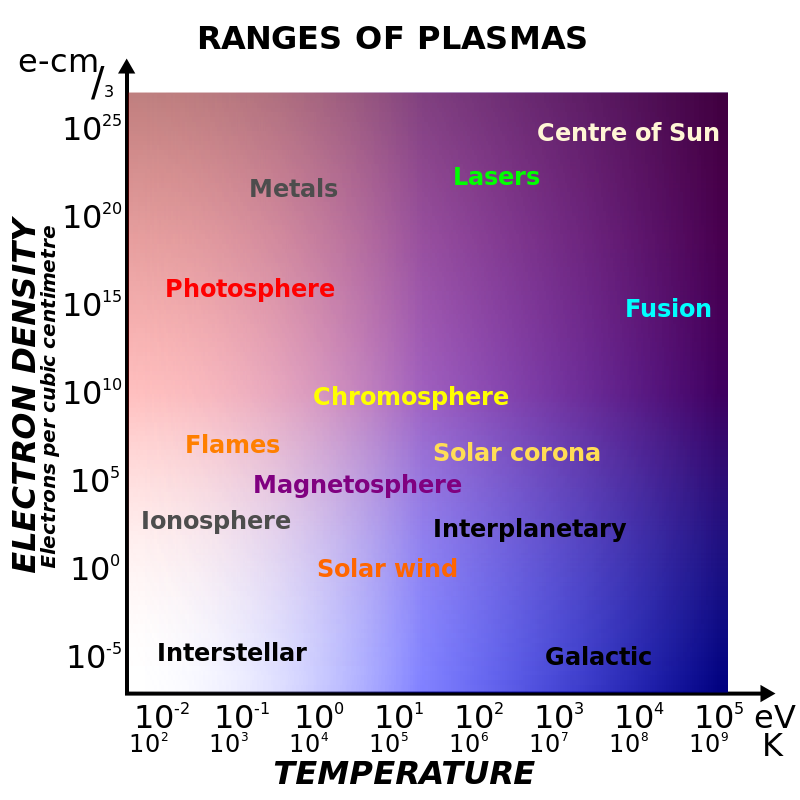
\includegraphics[scale=0.3]{faixaplasma.png}   
\caption{Aumento da densidade para cima, aumento da temperatura para a direita \cite{figplasma}.}
\label{fig: plasmafaixa}
\end{figure}

A magnetohidrodinâmica (MHD) é a área da física que estuda a interação mútua entre fluidos condutores e campos eletromagnéticos. 
Os fluidos em questão devem ser eletricamente condutivos e não magnéticos, ou seja, os limita a metais líquidos, eletrolitos fortes e o caso que estudaremos neste trabalho, o plasma. 
A interação mútua de um campo magnético $\bm{B}$ e um plasma de velocidade $\bm{u}$, surge como resultado das leis de Faraday e Ampère, devido a força de Lorentz.  
Dividindo este processo em três partes, temos basicamente que:
\begin{enumerate}
\item O movimento de um fluido condutor em um campo magnético provoca uma força eletromotriz induzida (de ordem $|\bm{u} \times \bm{B} | $) de acordo com a lei de indução de Faraday.  Em geral, correntes elétricas ocorrerão, sendo a densidade de corrente de ordem $\sigma (\bm{u} \times \bm{B})$, onde $\sigma$ é a condutividade elétrica. 
\item Estas correntes induzidas devem, de acordo com a lei de Ampère, dar origem a um campo magnético induzido que se soma ao campo magnético original, fazendo com que o fluido "arraste" \ as linhas do campo magnético junto com ele. 
\item O campo magnético combinado (imposto mais induzido) interage com a densidade de corrente induzida $\bm{J}$ para dar origem a uma densidade de força de Lorentz $\bm{J} \times \bm{B}$ que age no fluido condutor inibindo seu movimento no  campo magnético.  
\end{enumerate} 

Note que os dois últimos efeitos implicam em consequências semelhantes.  
Em ambos, o movimento do fluido no campo magnético tende a ser reduzido. 
Os fluidos podem \ "arrastar" \ linhas de campo magnético (efeito 2) e campos magnéticos podem puxar fluidos condutores (efeito 3). 
É esse "congelamento" \ parcial do meio e do campo magnético que é a marca registrada do modelo MHD ideal (a resistividade do plasma é nula).  

Para a descrição do plasma, são duas as abordagens mais comuns: o modelo de fluidos e o modelo cinético. 
Cada um com suas vantagens e desvantagens. %A magnetohidrodinâmica (MHD) é um caso particular do modelo de 1 fluido que descreve o plasma por meio de quantidades macroscópicas simplificadas, como por exemplo a  densidade numérica de partículas e a densidade de corrente.que são um caso particular das equações de um fluido quando as partículas não possuem carga elétrica 
O modelo de um fluido trata o plasma como um fluido único que é governado pelas equações do eletromagnetismo de Maxwell e as equações de Navier-Stokes, com a adição da força de Lorentz. 
%Portanto não levam em conta forças de origem eletromagnética. 

Neste trabalho, será usada uma descrição mais geral do plasma, ou seja, um modelo de dois fluidos. Neste modelo os íons e os elétrons são descritos como dois fluidos diferentes. %Com uma distribuição de velocidades para elétrons e outra para íons. 
Os modelos de fluidos são precisos quando a distribuição de velocidade das espécies se aproxima da distribuição de Maxwell-Boltzmann, o que normalmente ocorre quando o grau de colisões é alto, ou seja, um plasma quente onde o grau de ionização é alto. 
%Uma desvantagem do modelo de fluidos é que devido a descrição do plasma em termos de um único fluxo a uma determinada temperatura em cada localização espacial. 
%O modelo não permite capturar flutuações no plasma, como raios de luz ou camadas duplas, nem descrever efeitos ondulatórios de partículas. 
O modelo cinético não precisa assumir uma distribuição de Maxwell-Boltzmann, já que adota uma função de distribuição de velocidades em cada ponto do plasma. Porém, o modelo cinético demanda muito mais computação para ser resolvido satisfatoriamente. Devido a esse excessivo aumento de demanda computacional e de uma maior complexidade, escolhe-se normalmente para a modelagem do \textit{breakdown} o modelo de fluidos.


\section{Fusão} 
\noindent A fusão nuclear é um processo físico promissor para suprir a crescente demanda energética. 
O sol é alimentado por reações de fusão assim como todas as estrelas. 
Em tais reações, núcleos de baixa massa se combinam, ou se fundem, para formar núcleos mais massivos. 
No sol, uma sequência de reações de fusão, denominada cadeia p-p, começa com prótons - núcleos de hidrogênio comum - termina com partículas alfa - núcleos de átomos de hélio. Após uma reação de fusão, as massas finais são menores do que as iniciais e a diferença de massa é convertida em energia, através da conhecida equação de Einstein,
$$ E = \Delta m c^2 ,$$ 
onde $E$ é a energia resultante da reação, $\Delta m$ é a diferença de massa e $c$ é a velocidade da luz no vácuo. 
A fissão nuclear apresenta vários problemas, como riscos de explosões, produção significativa de resíduos radioativos e usos militares. 
O processo de fusão, no entanto, é naturalmente seguro, embora a reação de fusão também produza resíduos radioativos. No entanto, tais subprodutos são as partículas $\alpha$ (núcleos de Hélio). 
O fluxo de nêutrons em um reator tornará os materiais estruturais radioativos. 
O trítio tem uma meia-vida de apenas 12 anos, enquanto a escolha apropriada de materiais pode resultar em resíduos que têm meias-vidas de dezenas de anos, em vez de milhares de anos, como na fissão. 
Outra enorme vantagem da fusão é que os materiais usados para reação de fusão podem ser extraídas da água do mar. 
Portanto, a fusão é considerada uma fonte de energia virtualmente inesgotável. 
Como a fusão deve ser continuamente alimentada, e sua manutenção depende estritamente do equilíbrio MHD, ela é facilmente interrompida. 
Mesmo nos piores acidentes imagináveis, o plasma contido no tokamak não terá energia suficiente para causar a ruptura da câmera de vácuo.

\section{Tokamak} 
\noindent O tokamak é um conceito de máquina de confinamento de plasmas que tem como objetivo criar condições onde a fusão nuclear aconteça. 
A palavra tokamak é a transliteração de um acrônimo russo que significa "câmara toroidal com bobinas magnéticas". 
O objetivo final da pesquisa com tokamaks é tornar viável a construção de reatores nucleares de fusão com balanço positivo de energia, ou seja, a energia extraída é maior que a gasta para manter as reações de fusão. 
A reação de fusão mais promissora é a de deutério e trítio. 
A grande quantidade de energia liberada servirá para aquecer água, produzir vapor e assim mover uma turbina acoplada a um gerador elétrico. 
%A pesquisa em tokamaks, portanto, está ligada à procura de fontes alternativas de energia para a produção de eletricidade. 

Basicamente, um tokamak é um potente eletroímã que produz um campo magnético toroidal. 
Um toróide é a configuração mais simples com linhas de campo magnético fechadas, condição está necessária para evitar a perda do plasma. %no entanto, um campo puramente toroidal varia com $\frac{1}{R}$. 
O gradiente da amplitude do campo magnético e a curvatura das linhas de campo levam a movimentos de íons e elétrons em direções verticais opostas, o que resulta em uma separação de cargas. Esta, por sua vez, cria um campo elétrico que, junto com o campo magnético produzirá uma deriva das partículas na direção radial. %uma corrente elétrica. A geometria toroidal da corrente causa em lados opostos, correntes opostas causando uma força que tende a empurrar para fora todo o plasma. 
Este movimento de deriva para fora pode ser evitado torcendo as linhas do campo magnético, de modo que cada linha de campo passe pelas partes superior e inferior do toroide. 
De tal forma que a média ao longo do caminho das partículas leve a um cancelamento dos movimentos de desvio verticais e evite o estabelecimento de um campo elétrico. 
Portanto, uma combinação de campos magnéticos toroidais e poloidais pode adequadamente confinar um plasma.
No interior da câmera de vácuo de um tokamak ocorre uma emissão de elétrons que são altamente acelerados pelo campo elétrico, que então provocam uma ruptura (\textit{breakdown}) do gás de trabalho gerando a corrente de plasma, que irá formar o plasma que deve ser contido no espaço limitado da câmera de vácuo. 
O campo magnético não pode permitir que o plasma toque nas paredes internas da câmera de vácuo, tanto para não danificá-la, quanto para não dissipar a energia do plasma via condução térmica ou contaminar o plasma com átomos e moléculas pesadas. 
O tokamak é ainda caracterizado pela simetria azimutal. 
Alguns tokamaks tem sessão reta da câmera retangular, como o TCABR da USP, enquanto outros possuem sessão reta circular, como o NOVA-FURG, ou até alongada em formato elíptico, como o ITER. 
Outra característica dos tokamaks é o uso da corrente de plasma para gerar a componente helicoidal do seu intenso campo magnético, necessária para um equilíbrio MHD \cite[pg. 34]{tokamaks}, \cite[pg. 10]{MagneticControl}. 
A Figura \ref{fig: Rotulotokamak01} mostra os componentes básicos de um tokamak, onde os termos "Campo poloidal"\ e "Campo toroidal"\ se referem aos campos eletromagnéticos. 
No tokamak NOVA-FURG as duas bobinas de aquecimento ôhmico (em azul na Figura \ref{fig: Rotulotokamak001}) fazem o papel de enrolamento primário do transformador da Figura \ref{fig: Rotulotokamak01}, e a corrente de plasma faz o papel de enrolamento secundário do transformador.
Ao longo deste trabalho foi modelado no programa Blender o tokamak NOVA-FURG, respeitando as medidas de cada componente. O modelo pode ser visto na Figura \ref{fig: Rotulotokamak001} e uma imagem real da máquina na Figura \ref{fig: Rotulotokamak003}. 
O tokamak NOVA-FURG utiliza um núcleo de ferro como transformador ôhmico, possui uma parede de aço inox com uma camada condutora de alumínio e tratamento superficial da parede interna com titânio. E possui um filamento de tungstênio que fornece elétrons para ajudar no \textit{breakdown}.  
Detalhes dos parâmetros geométricos das bobinas do tokamak NOVA-FURG podem ser vistos na Tabela \ref{tab-nova} e na Figura \ref{fig: btokamak}. 
\begin{figure}[H]
\centering
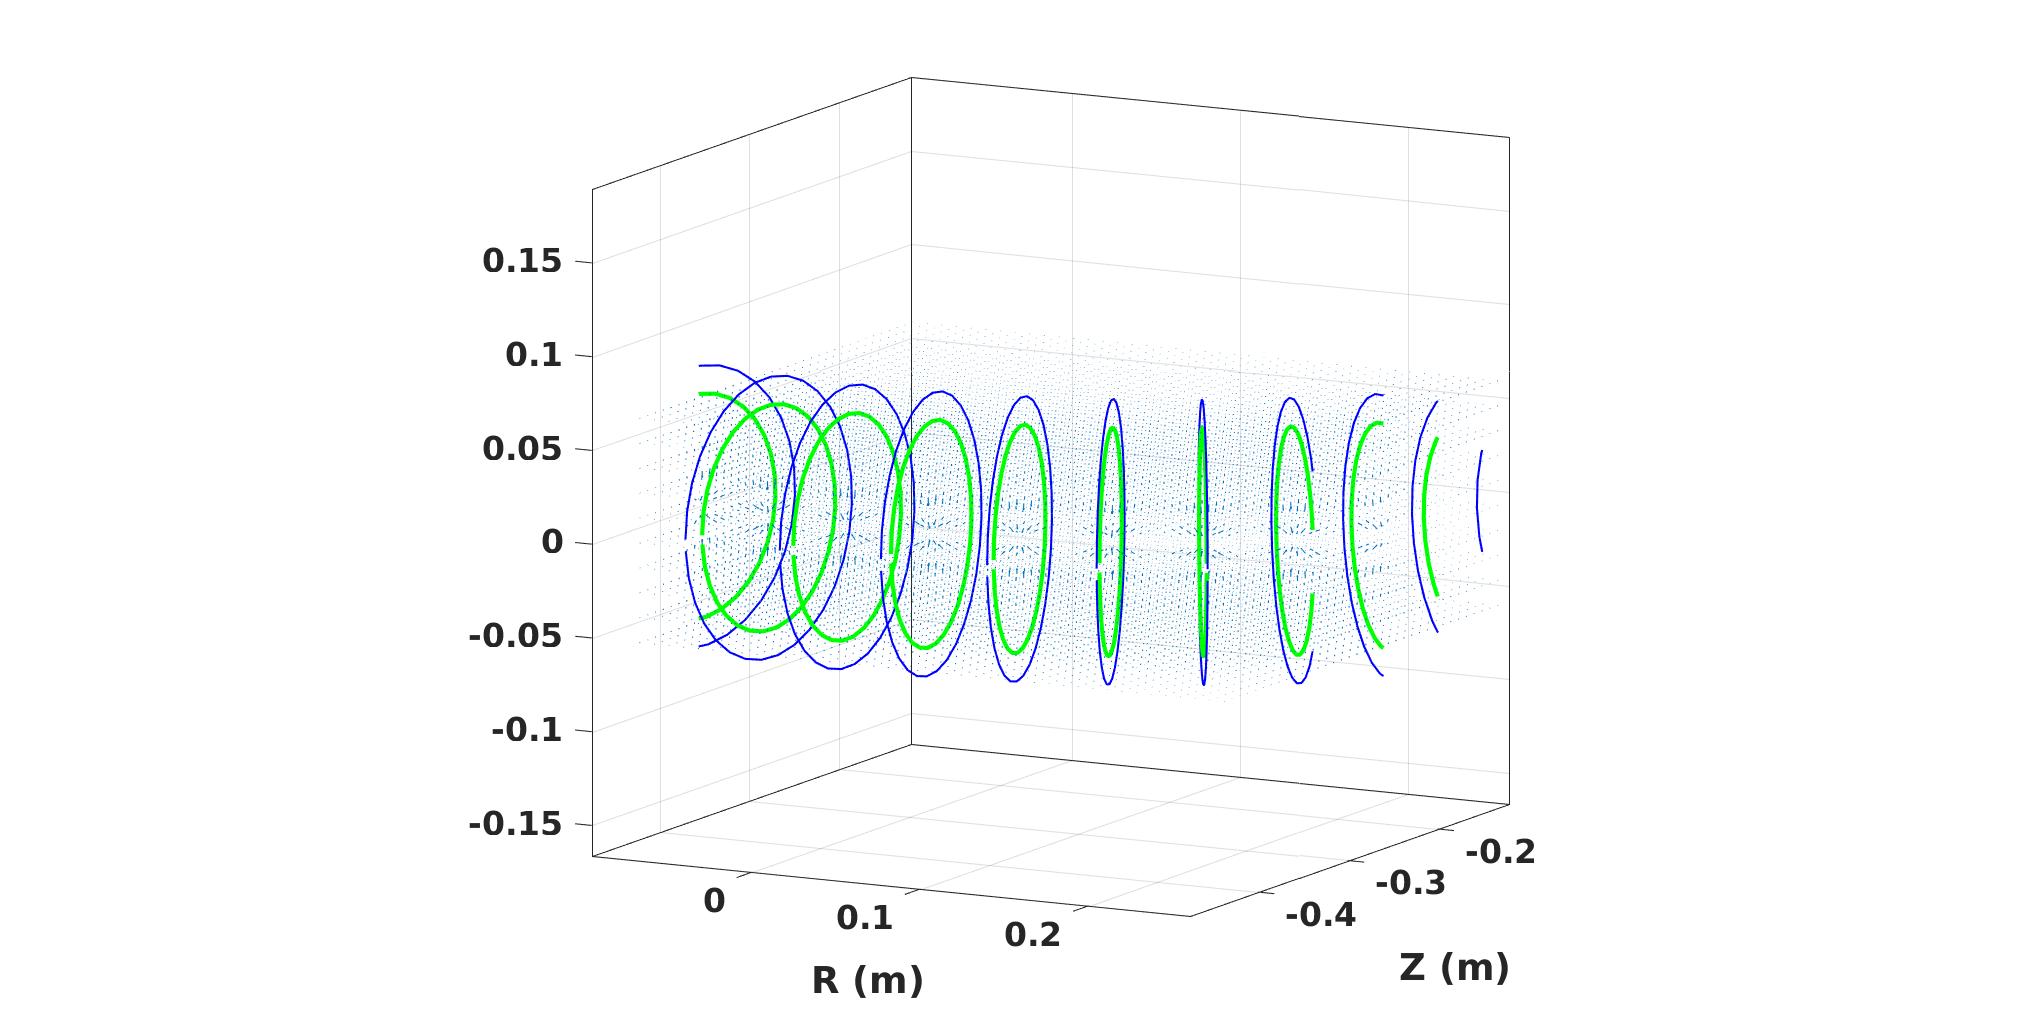
\includegraphics[scale=0.9]{../Rascunho_Resumo/tokamak.png} 
\caption{Esquema básico de um tokamak [Daltrini (1999), Ferrari e Nascimento (1988)].}
\label{fig: Rotulotokamak01}  
\end{figure}
\begin{figure}[H]
\centering
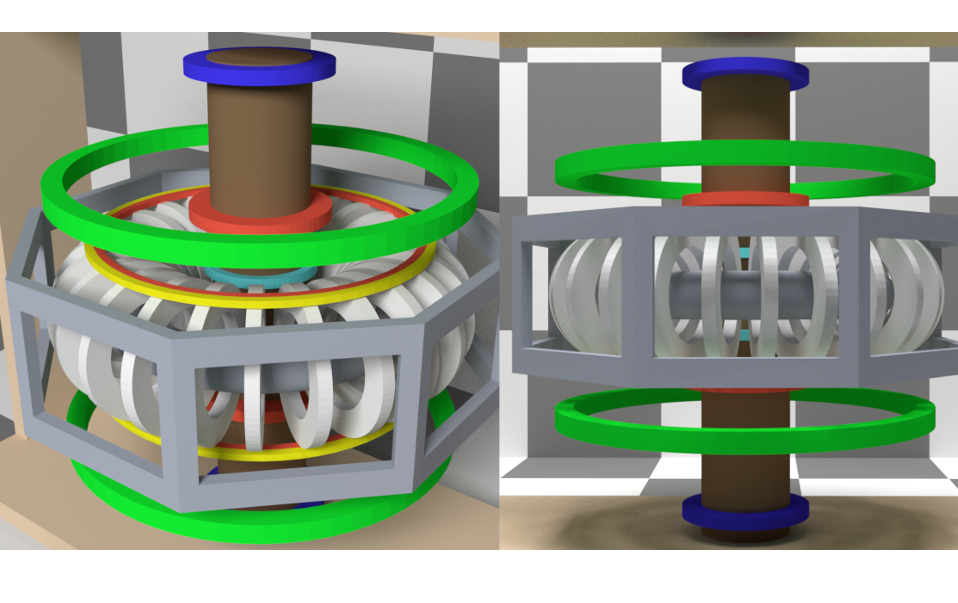
\includegraphics[scale=0.45]{tokamak12.png}
\caption{Tokamak NOVA-FURG, modelo feito no Blender.}    
\label{fig: Rotulotokamak001}
\end{figure}
\begin{figure}[H]
\centering
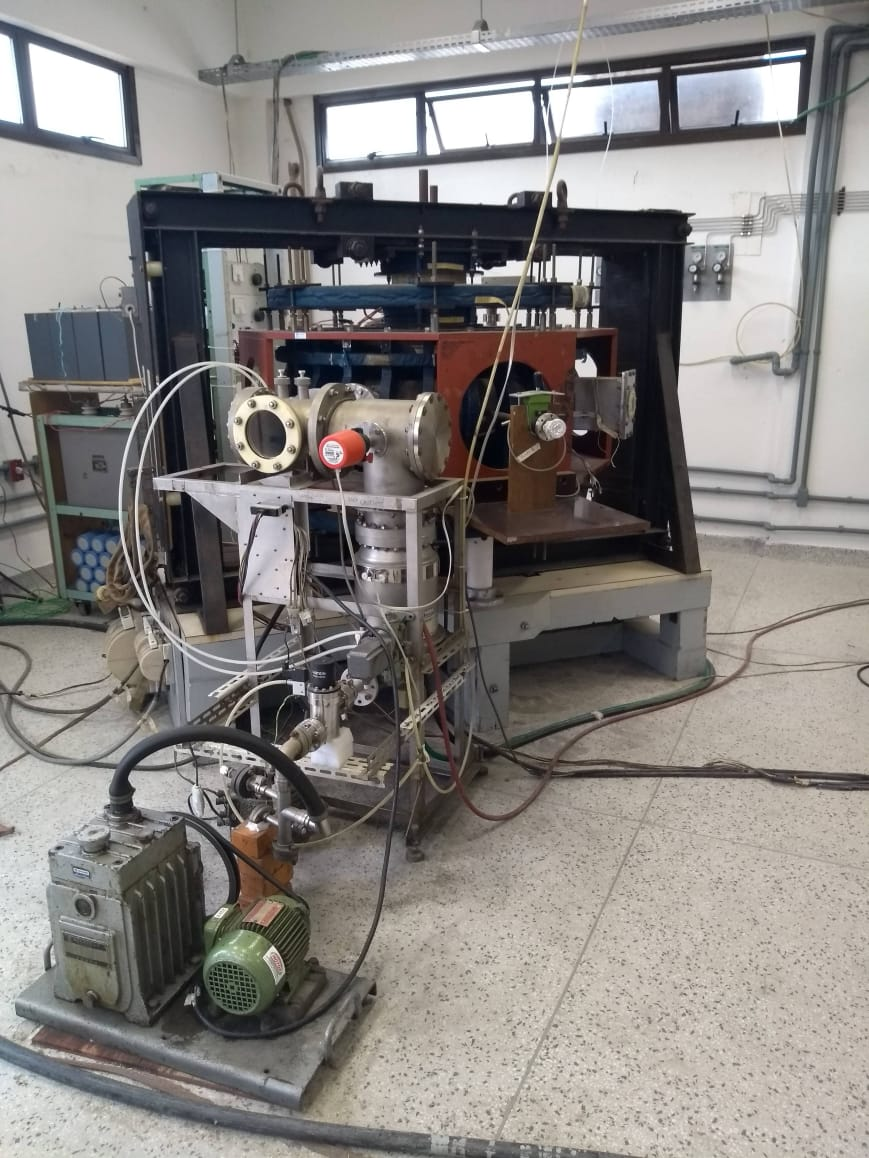
\includegraphics[scale=0.3]{../MPU19/tokamak.jpeg} 
\caption{Tokamak NOVA-FURG.}    
\label{fig: Rotulotokamak003}
\end{figure}
\section{Plasma \textit{startup}}
O início da operação de um tokamak consiste em três fases:
\begin{enumerate}
\item Fase de \textit{breakdown} do plasma (fase dominada pela avalanche de elétrons)
\item Fase de \textit{burn-through} (fase de ionização e aquecimento do plasma) 
\item Fase de \textit{current ramp-up} (estabelecimento da corrente de plasma).
\end{enumerate}
Na sequência, será dada uma breve descrição destas três fases, lembrando que o foco deste trabalho é a primeira fase. 

\subsection{Breakdown}
\noindent A fase de \textit{breakdown} em um tokamak é dominada por colisões entre elétrons livres e partículas neutras. A fase de \textit{breakdown} começa com a primeira ionização e dura até que as colisões de Coulomb comecem a dominar as colisões neutras com elétrons \cite[pg. 55]{sinha2017plasma}. %aqui foi pegado de referencia da pg 55 da tese brackdown e current formation
Este processo pode ser descrito pelo modelo desenvolvido por Townsend \cite{lloyd1991}. 
A descarga de Townsend (\textit{Townsend discharge}) é um processo de ionização de gás onde os elétrons livres, sob efeito de um campo elétrico intenso, são acelerados para então colidirem com moléculas de gás e liberarem elétrons adicionais, Figura \ref{avalanche}. 
Elétrons que também são acelerados, colidem e liberam mais elétrons adicionais, resultando em uma avalanche que permitirá a passagem de corrente pelo gás. Em um tokamak, o plasma parcialmente ionizado é condutor e uma corrente de plasma toroidal é formada devido ao campo elétrico toroidal.  
A descarga requer uma fonte de elétrons livres e um campo elétrico suficientemente intenso. 
O primeiro coeficiente de Townsend, explicado e modelado no apêndice \ref{Townsend}, corresponde ao número de reações de ionização, por unidade de comprimento, causadas por um elétron que se move paralelamente ao campo elétrico. 
O campo magnético poloidal, gerado pela corrente de plasma toroidal, começa a aumentar até que a corrente se estabiliza. 
São formadas então, superfícies de fluxo magnético fechadas que reduzem a perda de íons e elétrons, o que causa um aumento na taxa de crescimento da corrente de plasma. Uma explicação mais detalhada para a fase de \textit{breakdown} pode ser encontrada em \cite[pg. 40]{piras2011extremely}.

	\begin{figure}[H]
				\centering
			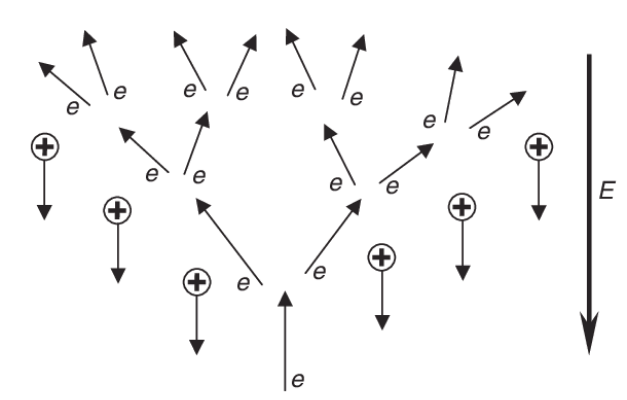
\includegraphics[scale=0.6]{avalanche.png} 
				\caption{Ilustração do breakdown de Townsend \cite{article0}.}
		\label{avalanche}
			\end{figure}
\subsection{Burn-through}
\label{burn-through}
%codigo usado para simular está fase: DYON (DYnamic0D model of Non-fully ionized plasma) code
\noindent A fase de \textit{burn-through} é caracterizada pelo aumento da corrente de plasma causada pelo aumento da ionização do plasma.
A ionização do gás neutro e radiações de linha das impurezas presentes no plasma, resultam na perda de uma parte significativa do poder de aquecimento \cite{breacdown, breacdown2}. Esta perda de potência é proporcional ao produto da densidade de elétrons com a densidade de partículas neutras, e tem seu máximo na chamada barreira de radiação. O plasma precisa "queimar" \ essa barreira de radiação antes que a potência de aquecimento possa elevar a temperatura do plasma. 
Um estado de alta ionização de impurezas é normalmente alcançado após a "queima" \ do gás principal. 
Uma "queima" \ (\textit{burn-through}) de plasma bem sucedida só pode ser obtida se a potência de aquecimento ôhmico exceder a perda de potência por ionização e radiação. 
Depois que a queima é realizada, a corrente de plasma é tipicamente aumentada até que o valor máximo de corrente de plasma (\textit{flattop}) seja atingido. 
Durante a fase de aceleração da corrente de plasma (\textit{ramp up} \ref{ramp-up}), é essencial evitar interrupções causadas por instabilidades MHD. 
As fases de \textit{breakdown}, \textit{burn-through} e \textit{ramp-up} não são necessariamente fases consecutivas, mas processos que podem ocorrer simultaneamente. 
É fundamental para o funcionamento do tokamak a obtenção da configuração de superfícies de fluxo fechado. Para isso, a corrente de plasma deve crescer e o gás combustível deve ser totalmente ionizado durante a fase de queima de plasma (\textit{burn-through}).
Uma das características cruciais na fase de \textit{burn-through} é a transição da configuração do campo magnético, ou seja, a mudança de configuração de linhas de campo abertas para as superfícies de fluxo fechadas. A Figura \ref{fig: burn-through} mostra dados típicos da fase de \textit{burn-through} no tokamak JET. Mais detalhes da fase de \textit{burn-through} podem ser encontrados em \cite{breacdown, kim2013plasma}.

\begin{figure}[h]
\centering
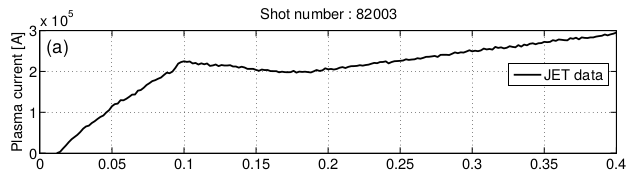
\includegraphics[scale=0.4]{burn-through-phase.png} 
\caption{Dados experimentais típicos de corrente de plasma medidos durante a fase de \textit{burn-through} no tokamak
JET \cite{kim2013physics}.}   
\label{fig: burn-through}
\end{figure}
%O código comumente usado na literatura para realizar simulações da fase de \textit{burn-through} é o DYON (DYnamic0D model of Non-fully ionized plasma).
\subsection{Ramp-up}
\label{ramp-up}
\noindent A fase de \textit{ramp-up} inicia-se após a queima do gás principal, mas é independente da quantidade de impurezas, podendo, então, se sobrepor à fase de \textit{burn-through}. A Figura \ref{fig: tokamakphases} apresenta um diagrama de como são caracterizadas, ao longo do tempo, as fases de \textit{breakdown}, \textit{burn-through} e \textit{ramp-up}.  Uma explicação mais detalhada para a fase de \textit{ramp-up} pode ser encontrada em \cite[pg. 49]{piras2011extremely}. A Figura \ref{fig: tokamakphases} apresenta um diagrama com as três fases ilustradas.

\begin{figure}[H]
\centering
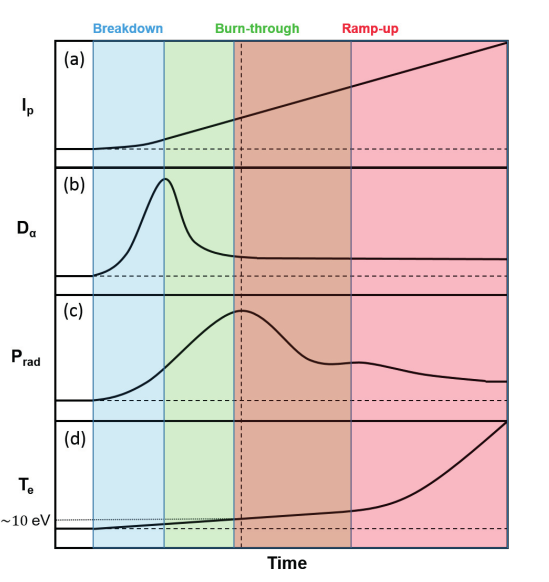
\includegraphics[scale=0.4]{tabela3fases.png}  
\caption{Figura esquemática da evolução temporal da (a) corrente de plasma, (b) emissão de $D_\alpha$, (c) perda de potência de radiação e ionização e (d) temperatura do elétron em uma formação típica de plasma de deutério. As fases de \textit{breakdown} (azul), \textit{burn-through} (verde), de \textit{ramp-up} (vermelho) e a sobreposição entre a fase de \textit{burn-through} e a fase de \textit{ramp-up} (marrom) são marcadas com as respectivas cores. A linha tracejada vertical representa a barreira de radiação \cite{sinha2017plasma}.}    
\label{fig: tokamakphases}
\end{figure}


\section{Função de distribuição}
\noindent A função de distribuição $f$ é uma função que contém informação sobre a densidade de partículas com posição entre $\bm{r}$ e $\bm{r}+d\bm{r}$ e velocidade entre $\bm{v}$ e $\bm{v}+d\bm{v}$. Definida num espaço de fase de seis dimensões, sendo três de posição e três de velocidade, a distribuição Maxwelliana \cite[pg. 127]{bittencourt} é dada por:
\begin{equation}
\label{distmax}
    f(\bm{r}, \bm{v}) = n(\bm{r}) \Big(\frac{m}{2\pi k_B T(\bm{r})}\Big)^{\frac{3}{2}}\exp\Big(\frac{-mv^2}{k_B T(\bm{r})}\Big),
\end{equation}
onde $n(\bm{r})$ é a densidade de partículas no espaço de configuração, $T(\bm{r})$ é a temperatura do plasma, $m$ é a massa das partículas, $\bm{v}$ é a velocidade e $k_B$ é a constante de Boltzmann. Quando o plasma está em equilíbrio termodinâmico a função de distribuição se torna Maxwelliana, conforme o teorema de Boltzmann.
Na maioria dos plasmas de laboratório, o estudo é feito fora do equilíbrio termodinâmico, uma vez que sempre se tem a variação de alguma propriedade macroscópica no plasma. Frequentemente estudos são feitos considerando que o plasma está em um certo equilíbrio, por exemplo elétrons estão em equilíbrio entre si a uma temperatura $T_e(\bm{r})$ e íons em equilíbrio entre si a uma temperatura $T_i(\bm{r})$. Investiga-se o que acontece com a distribuição a partir deste estado que se chama meta-equilíbrio.
A partir de $f$, obtemos a velocidade média
\begin{equation}
    <v> = \sqrt{\frac{8k_BT}{m\pi}},
    \end{equation} 
 a velocidade mais provável 
\begin{equation}
   v_{max}=\sqrt{\frac{2k_BT}{m}}
   \end{equation}   
e a velocidade quadrática média
\begin{equation}
   v_{rms}=\sqrt{\frac{3k_BT}{m}}.
   \end{equation} 
\section{Momentos da distribuição de Maxwell}
\noindent A função de distribuição é uma descrição microscópica de um plasma. Em contraste, uma descrição macroscópica de um plasma se faz pela especificação de valores médios das propriedades do plasma, tais como a densidade, velocidade média e pressão. A densidade de partículas da espécie $\alpha$ é dada por
\begin{equation*}
    n_\alpha(\bm{r},t) = \int_V f_\alpha(\bm{r},\bm{v},t) d^3 v,
\end{equation*}
a velocidade média das partículas da espécie $\alpha$ é
\begin{equation*}
    \bm{u}_\alpha(\bm{r},t) = \frac{1}{n_\alpha(\bm{r},t)} \int_V \bm{v} f_\alpha(\bm{r},\bm{v},t) d^3 v
\end{equation*}
e o tensor de pressão das partículas da espécie $\alpha$,
\begin{equation*}
    \mathbb{P}_\alpha(\bm{r},t) = \frac{m_\alpha}{n_\alpha(\bm{r},t)}\int_V (\bm{v}-\bm{u}_\alpha)(\bm{v}-\bm{u}_\alpha) f_\alpha(\bm{r},\bm{v},t) d^3 v,
\end{equation*}
onde $V$ é o espaço de velocidades.
%\int f_\alpha(\bm{r},\bm{v},t) \frac{d\bm{v}}{n_\alpha\bm{r}}

\chapter{Objetivos}
\noindent Na fase teórica deste trabalho pretende-se desenvolver um modelo de dois fluidos para o \textit{breakdown} em plasmas do tokamak NOVA-FURG. Para isso, primeiro temos de obter a equação geral dos momentos da equação de Boltzmann.
Após a dedução das equações para os três primeiros momentos da equação de Boltzmann, para elétrons e íons, o sistema será simplificado de acordo com as condições pertinentes a fase de \textit{breakdown} em tokamaks de pequeno porte. 
A fase computacional tem o propósito de resolver o sistema obtido na fase teórica, a fim de obter os parâmetros macroscópicos do plasma ao longo da fase de \textit{breakdown}, onde a corrente de plasma ainda é pequena permitindo que se admita que os campos elétrico e magnético gerados pelo plasma sejam nulos. 
Tendo então as distribuições ao longo dos tempos iniciais para os parâmetros do plasma, será verificado se os resultados condizem com o comportamento esperado do plasma.
Pretende-se após a realização das simulações numéricas interpretar fisicamente os resultados para cada variável macroscópica do modelo de 2 fluidos.  

\chapter{Revisão Bibliográfica}
\noindent Por volta de 1950 já existia alguns trabalhos sobre o modelo cinético e de fluidos. 
Nesta mesma época os físicos soviéticos Igor Tsamm e Andrei Sakharov sugeriram unir as pontas das máquinas líneares em um formato de toróide, visando melhorar o confinamento. 
Essa configuração foi chamada de tokamak. 
Ainda na mesma década, em 1958, Kruskal e  Kulsrud \cite{Kruskal1958} apresentaram algumas propriedades gerais do plasma usando as equações MHD, ou seja, equação da conservação da massa, do momento e da energia, juntamente com as equações de Maxwell e lei de Ohm. 
Ao longo de quase duas décadas, a pesquisa com o modelo de fluidos de plasmas confinados em tokamaks avançou muito. 
Em 1979 Hirshman e Jardin \cite{hirshman} publicam um artigo onde deduzem equações de transporte de dois fluidos. 
Dois anos depois é publicado por Sakanaka (1981) \cite{Sakanaka1981} uma dedução detalhada das equações de transporte a partir dos momentos da equação de Boltzmann. 

Com a construção de grandes tokamaks ao redor do mundo, os modelos de fluidos vieram a ser amplamente desenvolvidos para modelar o plasma nestes novos tokamaks. 
Foi usado por Zakharov e Rogers (1989-1993) \cite{Zakharov} um modelo linearizado de dois fluidos para a descrição do modo de \textit{kink} interno em tokamaks. 
Uma abordagem computacional baseada na evolução das equações de movimento de plasma eletromagnético, não linear e de dois fluidos foi usada por Thyagaraja (2000) \cite{Thyagaraja_2000} para investigar as propriedades da turbulência e do transporte do plasma tokamak. 
Pode-se ver mais detalhes sobre o \textit{breakdown} nos artigos de B. Lloyd, P. G. Carolan e C. D. Warrick (1996) \cite{breacdown} e D Mueller (2013) \cite{breacdown2}. 
Um estudo aprofundado juntamente com a realização de simulações numéricas das fases iniciais de operação de um tokamak é feito por Kim, Hyun Tae  \cite{kim2013physics} (2013). E por Sinha e Joyeeta \cite{sinha2017plasma} (2017) é feito um estudo aprofundado das três etapas iniciais do tokamak com muitos dados experimentais e comparações.  Em 1976 Hinton e Hazeltine \cite{RevModPhys.48.239} aprofundam o estudo sobre a teoria do transporte de plasma em sistemas de confinamento toroidal. Em 1989 Harafuji, Kenji, Hayashi, Takaya e Tetsuy \cite{harafuji1989computational} fizeram um estudo computacional dos equilíbrios MHD tridimensionais em sistemas helicoidais toroidais. Em \cite{weisstein2003toroidal}, o leitor pode conferir expressões em termos do seno e cosseno hiperbólico para os operadores diferenciais e em \cite{grimm1983ideal} pode-se conferir cálculos de estabilidade de MHD ideal em sistemas de coordenadas toroidais axissimétricos. Baseado nestes trabalhos será deduzido no apêndice \ref{pseudo-toroidaiss} o sistema de coordenadas pseudo-toroidais.

Como visto anteriormente, o uso dos modelos de fluidos é preferível em plasmas muito quentes e tem a vantagem de ser mais leve computacionalmente que os modelos cinéticos, como neste trabalho não iremos investigar efeitos microscópicos, um modelo de fluidos é o mais indicado. 


\begin{comment}
\chapter{Cronograma}
O cronograma do trabalho encontra-se na Tabela \ref{tab-cronograma}, onde as etapas são:

\begin{enumerate}
\item Levantamento bibliográfico;
\item Fase teórica:
\subitem Elaboração de uma introdução 
\subitem Dedução do modelo de 2 fluidos;
\subitem Simplificações cabíveis do modelo de 2 fluidos para o\textit{breakdown} no tokamak NOVA-FURG; 
\item Fase computacional:
\subitem Decidir a abordagem que será usada, se será explícita no tempo ou explícita e qual o melhor método numérico a ser usado no sistema;
\subitem  Implementação do modelo de 2 fluidos no MATLAB;
\subitem Definir as condições de contorno e fronteira;
\subitem Fazer diferentes simulações;
\item Análise dos resultados:
\subitem Relatório;
\subitem Síntese dos resultados;
\end{enumerate}

\begin{table}[h!]\begin{center}

	\begin{tabular*}{\textwidth}{@{\extracolsep{\fill}} c c c c c c c c c c c c}
		\toprule
		& Etapa & mar. & abr. & maio & jun. & jul. & ago. & set. & out. & nov. &\\
		\midrule
		&   1   &   x  &   x  &      &      &   x  &      &      &  x   &      &\\
		&   2   &   x  &   x  &   x  &   x  &      &      &      &      &      &\\
		&   3   &      &      &      &      &   x  &   x  &   x  &   x  &   x  &\\
		&   4   &      &      &      &      &      &      &      &   x  &   x  &\\
		\bottomrule                             
	\end{tabular*}
	\caption{Cronograma}\label{tab-cronograma}
\end{center}\end{table}

   \end{comment}

\chapter{Fase Teórica}
\label{faseteorica}
\noindent A fase teórica se inicia com uma dedução do modelo de 2 fluidos. 
Partindo da equação de Boltzmann, uma equação geral dos momentos é obtida, permitindo a dedução da equação de conservação da massa, do momento e da energia. 
O sistema de equações diferenciais parciais simplificado será escrito em termos da densidade de corrente. 
 
\section{Equação de Boltzmann}
\noindent De acordo com o modelo de fluidos, para descrever a dinâmica de um plasma, consideramos que os movimentos das partículas do plasma são governados pelos campos externos aplicados mais os campos internos gerados pelo plasma. O problema de obter o campo eletromagnético gerado pelo plasma, no entanto, ainda é complexo e requer uma solução auto-consistente com as equações de Maxwell.
A equação de Boltzmann é uma equação diferencial parcial usada para descrever a evolução temporal da função de distribuição $f_\alpha(\bm{r},\bm{v},t)$ no espaço das velocidades, posições e tempo. Em outras palavras, $f_\alpha(\bm{r},\bm{v},t)$ descreve a evolução temporal do sistema no espaço de fase \cite[pg. 193]{bittencourt}.
\begin{equation}
\label{eq: boltsmam}
\frac{\partial f_\alpha(\bm{r},\bm{v},t)}{\partial t} +\bm{v} \cdot \bm{\nabla} f_\alpha(\bm{r},\bm{v},t) + \bm{a} \cdot \bm{\nabla}_v f_\alpha(\bm{r},\bm{v},t) = \left( \frac{\delta f_\alpha}{\delta t} \right)_{coll} ,
\end{equation}   %\bm{C}_\alpha
onde $\bm{v}$ é a velocidade, $ \left( \frac{\delta f_\alpha}{\delta t} \right)_{coll} = \sum_\beta  \left( \frac{\delta f_\alpha}{\delta t} \right)_{\alpha \beta}$\{$f_\alpha$, $f_\beta$\} é o operador de colisão e os operadores diferenciais $\bm{\nabla}_v$ e $\bm{\nabla}$ em coordenadas cartesianas são 
$$\bm{\nabla}_v f_\alpha(\bm{r},\bm{v},t) =  \frac{\partial f_\alpha(\bm{r},\bm{v},t)}{\partial v_x} \hat{e}_{v_x} + \frac{\partial f_\alpha(\bm{r},\bm{v},t)}{\partial v_y} \hat{e}_{v_y} + \frac{\partial f_\alpha(\bm{r},\bm{v},t)}{\partial v_z} \hat{e}_{v_z}, $$  
$$\bm{\nabla} f_\alpha(\bm{r},\bm{v},t) = \frac{\partial f_\alpha(\bm{r},\bm{v},t)}{\partial x} \hat{e}_{x} + \frac{\partial f_\alpha(\bm{r},\bm{v},t)}{\partial y} \hat{e}_{y} + \frac{\partial f_\alpha(\bm{r},\bm{v},t)}{\partial z} \hat{e}_{z}$$
substituindo na eq. \ref{eq: boltsmam} os campos suavizados produzidos pelo plasma, obtêm-se então
\begin{equation}
\label{eq: boltzzz}
\frac{\partial f_\alpha(\bm{r},\bm{v},t)}{\partial t} +\bm{v} \cdot \bm{\nabla} f_\alpha(\bm{r},\bm{v},t) + \frac{1}{m_\alpha}[\bm{F}_{ext}+\bm{E}_{pl}+\bm{v} \times \bm{B}_{pl}] \cdot \bm{\nabla}_v f_\alpha(\bm{r},\bm{v},t)= \left( \frac{\delta f_\alpha}{\delta t} \right)_{coll},
\end{equation}
onde $\bm{F}_{ext}$ representa a força externa, incluindo a força de Lorentz associada a quaisquer campos elétrico e magnético aplicados externamente, e $\bm{E}_{pl}$ e $\bm{B}_{pl}$ são campos elétrico e magnético causados pela presença e movimento de todas as partículas carregadas dentro do plasma. Os campos eletromagnéticos $\bm{E}_{pl}$ e $\bm{B}_{pl}$  devem satisfazer as equações de Maxwell, uma vez que precisam ser consistentes com as densidades de carga e corrente macroscópicas existentes no próprio plasma
\begin{equation}
\label{eq: max1}
\bm{\nabla} \cdot \bm{E}_{pl} = \frac{\rho}{\epsilon_o},
\end{equation}
\begin{equation}
\label{eq: max2}
\bm{\nabla} \cdot \bm{B}_{pl} = 0,
\end{equation}
\begin{equation}
\label{eq: max3}
\bm{\nabla} \times \bm{E}_{pl} = -\frac{\partial \bm{B}_{pl}}{\partial t},
\end{equation}
\begin{equation}
\label{eq: max4}
\bm{\nabla} \times \bm{B}_{pl} = \mu_0 (\bm{J} + \epsilon_0 \frac{\partial \bm{E}_{pl}}{\partial t} ).
\end{equation}
Aqui $\mu_0 = 4\pi \times 10^{-7}$ [$N$ / $A^2$] é a permeabilidade magnética do vácuo, $\epsilon_0 = \frac{1}{\mu_0 c^2}$ é a permissividade elétrica do vácuo, $c$ a velocidade da luz no vácuo. 
A densidade de carga do plasma $\rho$ é dada por
\begin{equation}
\label{eq: rho}
\rho(\bm{r},t) = \sum_\alpha q_\alpha n_\alpha = \sum_\alpha q_\alpha \int_V f_\alpha(\bm{r},\bm{v},t) d^3v,
\end{equation}
e a densidade de corrente de plasma $\bm{J}$ é dada por
\begin{equation}
\label{eq: densidadecorrente}
\bm{J}(\bm{r},t) = \sum_\alpha q_\alpha n_\alpha \bm{u}_\alpha(\bm{r},t) = \sum_\alpha  q_\alpha \int_V \bm{v} f_\alpha(\bm{r},\bm{v},t) d^3v.
\end{equation}
Aqui $ \bm{u}_\alpha(\bm{r},t)$ denota a velocidade macroscópica do fluido (apêndice \ref{anexo1}). As equações eq. \ref{eq: boltzzz}, eq. \ref{eq: max1}, eq. \ref{eq: max2}, eq. \ref{eq: max3}, eq. \ref{eq: max4}, eq. \ref{eq: rho} e eq. \ref{eq: densidadecorrente} constituem um conjunto completo de equações a serem resolvidas ao mesmo tempo. %Então, por exemplo, em um procedimento iterativo, assumindo valores aproximados iniciais para $\bm{E}_{pl}(\bm{r}, t)$ e $\bm{B}_{pl}(\bm{r}, t)$, a eq. \ref{eq: boltzzz} pode ser resolvida para produzir $f_\alpha(\bm{r},\bm{v},t)$ para os tipos diferentes de partículas. A utilização dos valores calculados na eq. \ref{eq: rho} e eq. \ref{eq: densidadecorrente} leva a valores para as densidades de carga e corrente no plasma, que podem ser substituídas nas equações de Maxwell e resolvidas para $\bm{E}_{pl}(\bm{r}, t)$ e $\bm{B}_{pl}(\bm{r}, t)$. Esses valores são então introduzidos novamente na equação de Boltzmann (eq. \ref{eq: boltzzz}), e assim por diante, para obter uma solução auto-consistente para a função de distribuição de partículas individuais. %Embora a equação eq. \ref{eq: boltzzz} não inclua explícitamente um termo de colisão no seu lado direito e portanto, não leve em consideração colisões de curto alcance, ela é mais geral do que parece, já que uma considerável parte dos efeitos de interações de partículas já foram incluídas na força de Lorentz, por meio dos campos eletromagnéticos suavizados auto-consistentes internos. 
Não é necessário resolver a equação de Boltzmann para encontrar as variáveis macroscópicas de interesse físico. Estas variáveis estão relacionadas com os momentos da equação de Boltzmann. %As equações de transporte podem ser obtidas tomando os momentos da equação de Boltzmann. 



\section{Momentos da distribuição}
\noindent Nesta sessão, será obtida da equação de Boltzmann, a equação geral dos momentos. 
Seja uma propriedade física $\chi(v)$ das partículas do plasma. Multiplicando cada termo da eq. \ref{eq: boltzzz} por $\chi(v)$ e integrando a equação resultante sobre todo o espaço de velocidade obtemos

\begin{equation}
\label{eq: pit3.01}
\int_V \chi \frac{\partial f_\alpha}{\partial t} d^3 v + \int_V \chi \bm{v} \cdot \bm{\nabla} f_\alpha d^3 v + \int_V \chi \bm{a} \cdot \bm{\nabla}_v f_\alpha d^3 v = \int_V \chi \left( \frac{\delta f_\alpha}{\delta t} \right)_{coll} d^3 v.
\end{equation}
Resolvendo cada integral separadamente,

\begin{equation}
\label{eq: pit4.01}
\int_V \chi \frac{\partial f_\alpha}{\partial t} d^3 v  = \frac{\partial }{\partial t} (\int_V \chi f_\alpha d^3 v)-\int_V \frac{\partial \chi}{\partial t} f_\alpha d^3 v.
\end{equation}
No entanto, desde que $\chi = \chi(\bm{v})$, sua derivada parcial em relação ao tempo é zero. Usando a definição de valores médios (anexo \ref{anexo1}), o rendimento fica
\begin{equation}
\label{eq: pit5.01}
\int_V \chi \frac{\partial f_\alpha}{\partial t} d^3 v = \frac{\partial}{\partial t} [n_\alpha<\chi>_\alpha],
\end{equation}

\begin{equation}
\label{eq: pit6.01}
\int_V \chi \cdot \bm{v} \bm{\nabla} f_\alpha d^3 v = \bm{\nabla} \cdot \left( \int_V \chi \bm{v} f_\alpha d^3 v \right) - \int_V \bm{\nabla} \chi \cdot \bm{v} f_\alpha d^3 v - \int_V \chi  f_\alpha \bm{\nabla} \cdot \bm{v}  d^3 v.
\end{equation}
Como visto anteriormente, $\chi = \chi(\bm{v})$, então seu gradiente é zero e as variáveis $\bm{r}$, $\bm{v}$ e $t$ são independentes, então o divergente de $\bm{v}$ também é zero, resultando em
\begin{equation}
\label{eq: pit7}
\int_V \chi \bm{v} \cdot \bm{\nabla} f_\alpha d^3 v = \bm{\nabla} \cdot [n_\alpha<\chi \bm{v}>_\alpha],
\end{equation}
\begin{equation}
\label{eq: pit8}
\int_V \chi \bm{a} \cdot \bm{\nabla}_v f_\alpha d^3 v = \int_V \bm{\nabla}_v \cdot (\bm{a} \chi f_\alpha)d^3 v - \int_V f_\alpha (\bm{a} \cdot \bm{\nabla}_v \chi) d^3 v - \int_V \chi  f_\alpha (\bm{\nabla}_v \cdot \bm{a})  d^3 v.
\end{equation}
A primeira integral desaparece porque a função de distribuição deve desaparecer para $\pm \infty$. A última integral na eq. \ref{eq: pit8} desaparece se assumirmos que
\begin{equation}
\label{eq: pit9}
\bm{\nabla}_v \cdot \bm{a} = \frac{1}{m_\alpha} \bm{\nabla}_v \cdot \bm{F} = 0,
\end{equation}
isto é, se o componente de força $F_j$ for independente do componente de velocidade correspondente $v_j$, uma vez que $\bm{\nabla}_v \cdot \bm{F} = \sum_j \frac{\partial F_j}{\partial v_j}$. Isto é verdade para a força devido a um campo magnético, $\bm{F} = q_\alpha \bm{v} \times \bm{B}$ porque $j$ também neste caso $F_j$ é independente de $v_i$.
\begin{equation}
\label{eq: pit10}
\int_V \chi \bm{a} \cdot \bm{\nabla}_v f_\alpha d^3 v = -n_\alpha<\bm{a} \cdot \bm{\nabla}_v \chi>_\alpha,
\end{equation}
\begin{equation}
\label{eq: pit11}
\int_V \chi \left( \frac{\delta f_\alpha}{\delta t} \right)_{coll} d^3 v = \left[\frac{\delta}{\delta t}(n_\alpha<\chi>_\alpha)\right].
\end{equation}
Combinando as eq. \ref{eq: pit5.01}, eq. \ref{eq: pit7}, eq. \ref{eq: pit10} e eq. \ref{eq: pit11} na eq. \ref{eq: pit3.01} obtemos finalmente 
\begin{equation}
\label{eq: pit12}
\frac{\partial }{\partial t}(n_\alpha<\chi>_\alpha) + \bm{\nabla} \cdot (n_\alpha<\chi \bm{v} >_\alpha) - n_\alpha<\bm{a} \cdot \bm{\nabla}_v \chi>_\alpha = 
\end{equation}
\begin{equation*}
=[\frac{\delta}{\delta t}(n_\alpha<\chi>_\alpha)].
\end{equation*}
Que é a equação geral dos momentos. Na sequência serão obtidas, através da equação geral dos momentos, as equações de conservação da massa, do momento e da energia.
\section{Modelo de um fluido}
Primeiro resolveremos uma versão mais simples, o modelo de um fluido sem ionização:
\begin{eqnarray}
&\label{eq:one}
\frac{\partial}{\partial t}n + \bm{\nabla} \cdot \big( n \bm{u} \big)  = 0, \\
%momentun
&\label{eq:two}
m n \left[ \frac{\partial}{\partial t} + \bm{u} \cdot  \bm{\nabla} \right] = \bm{J} \times \bm{B} -\bm{\nabla}p,\\  
%energy conservation
&\label{eq:five}
\bm{\nabla}p=V_s^2 \nabla \big( nm \big),\\
&\label{eq:six}
\bm{\nabla} \times \bm{E}= -\frac{\partial}{\partial t} \bm{B},\\
&\label{eq:seven}
\bm{\nabla} \times \bm{B}=\mu_0 \bm{J},\\
&\label{eq:eigh}
\bm{J}=\sigma_0 \big( \bm{E}+ \bm{u} \times \bm{B} \big) -\frac{\sigma_0}{n e} \bm{J} \times \bm{B}.
\end{eqnarray}
onde $\sigma_0=\frac{n e^2}{me \nu_{ei}}$. A equação \ref{eq:one} está igualada a 0 oque seiguinifica que não temos ionização. A equação da energia simplificou para \ref{eq:five}. 
Remember that:
\begin{equation*}
\bm{\nabla} \times \bm{F} =  \left[\frac{1}{r} \frac{\partial F_z}{\partial \phi} - \frac{\partial F_\phi}{\partial z} \right]  \hat{e}_r + \left[  \frac{\partial F_r}{\partial z} -  \frac{\partial F_z}{\partial r}  \right] \hat{e}_\phi + \left[ \frac{1}{r} \frac{\partial}{\partial r}\Big( r F_\phi \Big) - \frac{1}{r} \frac{\partial F_r}{\partial \phi}  \right] \hat{e}_z.
\end{equation*} 
Agora simplificando e abrindo nos componentes dos vetores
\begin{eqnarray}
&\label{eq:one2}
\dfrac{\partial n}{\partial t} + \frac{1}{r} \left( \dfrac{\partial \big( rn \big)}{\partial r} u_r+\dfrac{\partial u_r }{\partial r} nr \right)+\dfrac{\partial n}{\partial z} u_z+\dfrac{\partial u_z}{\partial z} n = 0, \\
%momentun
&\label{eq:two2}
m n \left[ \dfrac{\partial n}{\partial t} + \frac{1}{r} \dfrac{\partial \big( r u_r \big)}{\partial r} +\dfrac{\partial u_z}{\partial z} \right] =\left( \begin{array}{c}
 J_z B_r - J_r B_z  \\
 J_z B_r - J_r B_z  \\
 J_r B_\phi - J_\phi B_r 
\end{array} \right)
-\left( \dfrac{\partial p}{\partial r} +\dfrac{\partial p}{\partial z}\right)\\  
%energy conservation
&\label{eq:five2}
\left( \dfrac{\partial p}{\partial r} +\dfrac{\partial p}{\partial z}\right)=m V_s^2 \left( \dfrac{\partial n}{\partial r} +\dfrac{\partial n}{\partial z}\right) ,\\
&-\dfrac{\partial E_\phi}{\partial z}   = -\dfrac{\partial B_r}{\partial t} ,\nonumber\\
& \label{eq:six2} 
\dfrac{\partial E_r}{\partial z} -  \dfrac{\partial E_z}{\partial r}  =-\dfrac{\partial B_\phi}{\partial t}, \\
& \frac{1}{r} \dfrac{\partial}{\partial r}\big( r E_\phi \big)  =-\dfrac{\partial B_z}{\partial t} ,\nonumber \\
%%%%%%
&-\dfrac{\partial B_\phi}{\partial z}   = \mu_0 J_r ,\nonumber\\
& \label{eq:seven2} 
\dfrac{\partial B_r}{\partial z} -  \dfrac{\partial B_z}{\partial r}  =\mu_0 J_\phi, \\
& \frac{1}{r} \dfrac{\partial}{\partial r}\big( r B_\phi \big)  = \mu_0 J_z,\nonumber \\
%%%
& J_r= \sigma_0 \Big( E_r+ \left[ u_\phi B_z - u_z B_\phi \right] \Big)-\frac{\sigma_0}{n e} \left[ J_\phi B_z - J_z B_\phi \right] , \nonumber\\
&\label{eq:eigh2}
J_\phi = \sigma_0 \Big( E_\phi+ \left[ u_z B_r - u_r B_z \right] \Big)-\frac{\sigma_0}{n e} \left[ J_z B_r - J_r B_z \right] ,\\
& J_z=\sigma_0 \Big( E_z+ \left[ u_r B_\phi - u_\phi B_r \right] \Big)-\frac{\sigma_0}{n e} \left[ J_r B_\phi - J_\phi B_r \right]. \nonumber
\end{eqnarray}
%\sigma_0 \big( \bm{E}+ \bm{u} \times \bm{B} \big) -\frac{\sigma_0}{n e} \bm{J} \times \bm{B},
\section{Equação de conservação da massa}
\noindent A equação de conservação da massa, também conhecida como equação da continuidade, garante que toda massa ganha ou perdida pelo sistema é quantificada no termo $S_\alpha$.
Essa equação pode ser obtida diretamente pela substituição, na eq. \ref{eq: pit12} do $\chi$ por $m_\alpha$. 
Definindo a densidade de massa como $ \rho_{m\alpha} = n_\alpha m_\alpha$ temos
\begin{equation}
\label{eq: pit13}
\frac{\partial \rho_{m\alpha}}{\partial t} + \bm{\nabla} \cdot (\rho_{m\alpha} \bm{u}_\alpha)  = S_\alpha, 
\end{equation}
onde o termo de colisão, $S_\alpha = \left[\frac{\delta \rho_{m\alpha}}{\delta t}\right]_{coll}$, representa a taxa na qual partículas do tipo $\alpha$ são produzidas ou perdidas, por unidade de volume, como resultado de colisões, de acordo com \cite[pg. 197]{bittencourt}.
Seja $\rho_\alpha(\bm{r},t)$ a densidade de carga dada por $\rho_\alpha(\bm{r},t)=n_\alpha q_\alpha$ e $\bm{J}_\alpha$ a densidade de corrente, dada por $\bm{J}_\alpha=\rho_\alpha \bm{u}_\alpha$, podemos reescrever a eq. \ref{eq: pit13} em termos da densidade de corrente se dividirmos a eq. \ref{eq: pit13} por $m_\alpha$ e  multiplicarmos por $q_\alpha$ obtendo a equação de conservação da carga elétrica
\begin{equation}
\label{eq: pit13.001}
\frac{\partial \rho_{\alpha}}{\partial t} + \bm{\nabla} \cdot \bm{J}_\alpha  = \frac{q_\alpha}{m_\alpha} S_\alpha.
\end{equation}
 
\section{Equação de conservação do momento}
\noindent A equação de conservação do momento afirma que a taxa de mudança do momento de um fluido $\alpha$ é devida às forças externas aplicadas no fluido, à força de pressão do próprio fluido e também pelas forças internas devido a colisões, dispersão e produção de partículas de plasma.
Para derivar a equação de conservação do momento, $\chi$ é substituído por $m_\alpha \bm{v}_\alpha$ na eq. \ref{eq: pit12}, ou seja,
\begin{equation}
\label{eq: p2}
\frac{\partial }{\partial t}(n_\alpha<m \bm{v}>_\alpha) + \bm{\nabla} \cdot (n_\alpha<m \bm{v}^2 >_\alpha) 
\end{equation}
\begin{equation*}
= n_\alpha<\bm{a} \cdot \bm{\nabla}_v m \bm{v}>_\alpha +[\frac{\delta}{\delta t}(n_\alpha<m \bm{v}>_\alpha)].
\end{equation*}
Definindo $\bm{v}_\alpha = \bm{c}_\alpha + \bm{u}_\alpha$, onde $\bm{c}_\alpha$ é a velocidade térmica das partículas e  $\bm{u}_\alpha$ é a velocidade do fluido. 
Vamos tratar de cada termo da eq. \ref{eq: p2} separadamente.
Aplicando a definição de valor médio (apêndice \ref{anexo1}) e como $ \rho_{m\alpha} = n_\alpha m_\alpha$, ficamos com $\frac{\partial }{\partial t} (n_\alpha <\chi>_\alpha)=\frac{\partial }{\partial t} (n_\alpha <m \bm{v}>_\alpha)$, mas $\bm{c}_\alpha$ não influencia no valor médio. Portanto, ficamos com $\frac{\partial }{\partial t} (\rho_{m\alpha} \bm{u}_\alpha)$. 
Aplicando a regra da cadeia na derivada parcial obtemos
\begin{equation}
\label{eq: pit14}
\frac{\partial }{\partial t} (\rho_{m\alpha} \bm{u}_\alpha) = \bm{u}_\alpha \frac{\partial \rho_{m\alpha}}{\partial t}+\rho_{m\alpha} \frac{\partial \bm{u}_\alpha}{\partial t}.
\end{equation} 
Substituindo $\chi$ pelo momento $m_\alpha \bm{v}_\alpha$ temos $\bm{\nabla} \cdot (n_\alpha <\chi \bm{v}>_\alpha) =  \bm{\nabla} \cdot (n_\alpha <m \bm{v} \bm{v}>_\alpha)$ e tirando $m_\alpha$ para fora da média, pois é constante, temos $\bm{\nabla} \cdot (n_\alpha m_\alpha < \bm{v} \cdot \bm{v}>_\alpha)$. %Nota-se que dentro do termo de média, $ \bm{v}_\alpha$ é igual $\bm{v}$, pois o tipo de partícula $\alpha$ já está representado na operação valor médio $< >_\alpha$, produzindo $\bm{\nabla} \cdot (\rho_{m\alpha} <\bm{v} \cdot \bm{v}>)$. 
Aplicando a definição de valor médio obtemos 
\begin{equation}
\label{eq: pit15}
\bm{\nabla} \cdot (\rho_{m\alpha} <\bm{v} \cdot \bm{v}>) = \bm{\nabla} \cdot ( \rho_{m\alpha}\bm{u}_\alpha \cdot \bm{u}_\alpha + \rho_{m\alpha}<\bm{c} \cdot \bm{c}>_\alpha)
\end{equation} 
já que $\bm{c} \cdot \bm{u} = 0$, uma vez que $\bm{c}$ é isotrópico e não contribui para o valor médio de $\bm{v}_\alpha$ que, por definição, é igual a $\bm{u}_\alpha$.  %vai em todas as direções
No termo seguinte, $n_\alpha<\bm{a} \cdot \bm{\nabla}_v m_\alpha \bm{v}>_\alpha$, rearranjamos os termos ficando com $n_\alpha<(m_\alpha \bm{a} \cdot \bm{\nabla}_v) \bm{v}>_\alpha$. Observando que massa vezes aceleração é força, $\bm{F} = \bm{a} \cdot m_\alpha $, temos $n_\alpha <(\bm{F} \cdot \bm{\nabla}_v)\bm{v}>_\alpha$, que nos da
\begin{equation}
\label{eq: pit16}
n_\alpha <(\bm{F} \cdot \bm{\nabla}_v)\bm{v}>_\alpha=n_\alpha<\bm{F}>_\alpha,
\end{equation}
pois $(\bm{F} \cdot \bm{\nabla}_v)\bm{v} = \bm{F} \cdot (\bm{\nabla}_v\bm{v})$ e $\bm{\nabla}_v\bm{v} = 1$. 
Definindo $\bm{R}_\alpha$ como sendo a soma da taxa de mudança de momento devido ao espalhamento com a taxa de mudança de momento devido à produção de partículas \cite[pg. 201]{bittencourt}, obtemos
\begin{equation}
\label{eq: pit17}
\bm{R}_\alpha = \left[\frac{\delta}{\delta t}(n_\alpha<m \bm{v}>_\alpha)\right]=\left[\frac{\delta}{\delta t}(\rho_{m\alpha}\bm{u}_\alpha)\right].
\end{equation}
Substituindo eq. \ref{eq: pit14}, eq. \ref{eq: pit15}, eq. \ref{eq: pit16}, eq. \ref{eq: pit17} em eq. \ref{eq: p2} obtemos
\begin{equation}
\label{eq: pit19}
\bm{u}_\alpha \frac{\partial \rho_{m\alpha}}{\partial t} + \rho_{m\alpha} \frac{\partial \bm{u}_\alpha}{\partial t}+ \bm{\nabla} \cdot (\rho_{m\alpha} \bm{u}_\alpha \bm{u}_\alpha)+
\end{equation} 
\begin{equation*}
+\bm{\nabla} \cdot (\rho_{m\alpha} <\bm{c} \cdot \bm{c}>_\alpha)-n_\alpha<\bm{F}>_\alpha=\bm{R}_\alpha.
\end{equation*}
Definindo o tensor $\mathbb{P}_\alpha=\rho_{m\alpha} <\bm{c} \cdot \bm{c}>_\alpha$, que representa a força por unidade de volume dentro do plasma devido aos movimentos aleatórios das partículas \cite[pg. 149]{bittencourt}, temos que
\begin{equation}
\label{eq: pit20}
\bm{\nabla} \cdot (\rho_{m\alpha} \bm{u}_\alpha \bm{u}_\alpha) =  \rho_{m\alpha}(\bm{u}_\alpha \cdot \bm{\nabla})\bm{u}_\alpha + [\bm{\nabla} \cdot (\rho_{m\alpha} \bm{u}_\alpha)]\bm{u}_\alpha.
\end{equation}
Fazendo a força igual a força de Lorentz temos 
\begin{equation}
\label{eq: pit20.1}
<\bm{F}>_\alpha = q_\alpha (\bm{E} + \bm{u}_\alpha \times \bm{B})
\end{equation} e substituindo as eq. \ref{eq: pit20} e eq. \ref{eq: pit20.1} em eq. \ref{eq: pit19}, teremos
\begin{equation}
\label{eq: pit21}
 \bm{u}_\alpha \frac{\partial \rho_{m\alpha}}{\partial t} + \rho_{m\alpha} \frac{\partial \bm{u}_\alpha}{\partial t}+ \rho_{m\alpha} (\bm{u}_\alpha \cdot \bm{\nabla})\bm{u}_\alpha+[\bm{\nabla} \cdot (\rho_{m\alpha} \bm{u}_\alpha)]\bm{u}_\alpha  =
\end{equation}
\begin{equation*}
n_\alpha q_\alpha (\bm{E} + \bm{u}_\alpha \times \bm{B})-\bm{\nabla} \cdot \mathbb{P}_\alpha + \bm{R}_\alpha.
\end{equation*}
Rearranjando estes termos, temos que
\begin{equation}
\label{eq: pit22}
\rho_{m\alpha} \left[\frac{\partial \bm{u}_\alpha}{\partial t} + (\bm{u} \cdot \bm{\nabla})\bm{u}_\alpha \right]+ \bm{u}_\alpha \left[ \frac{\partial \rho_{m\alpha}}{\partial t} + \bm{\nabla} \cdot (\rho_{m\alpha} \bm{u}_\alpha)  \right] = 
\end{equation}
\begin{equation*}
=\bm{R}_\alpha +n_\alpha q_\alpha (\bm{E} + \bm{u}_\alpha \times \bm{B})-\bm{\nabla} \cdot \mathbb{P}_\alpha.
\end{equation*}
No entanto, o segundo termo no lado esquerdo da eq. \ref{eq: pit22} é a equação de conservação de massa eq. \ref{eq: pit13}, %então se não considerarmos as colisões que levam à geração ou perda de partículas, ou seja $S_\alpha = 0$, podemos simplificar a equação para (se sp for zero \bm{R} também será pois ambos são devido à colisões) (isotropica: não à direção privilegiada, suas propriedades são as mesmas em qualquer direção)
\begin{equation}
\label{eq: pit23}
\rho_{m\alpha} \left[\frac{\partial \bm{u}_\alpha}{\partial t} + (\bm{u} \cdot \bm{\nabla})\bm{u}_\alpha \right] =  \bm{R}_\alpha+n_\alpha q_\alpha (\bm{E} + \bm{u}_\alpha \times \bm{B})-\bm{\nabla} \cdot \mathbb{P}_\alpha-\bm{u}_\alpha S_\alpha.
\end{equation}
O termo $-\bm{\nabla} \cdot \mathbb{P}_\alpha $ representa a força causada pelas variações aleatórias nas velocidades de cada partícula que é exercida em um volume unitário do plasma. 
Esta força em cada unidade de volume também inclui forças associadas à pressão escalar e forças de cisalhamento, que são as forças viscosas. No nosso caso, o efeito da viscosidade é pequeno de modo que os termos não-diagonais de $\mathbb{P}_\alpha$ podem ser desprezados. 
Além disso, no caso em que a distribuição de velocidades de cada tipo de partícula é isotrópica, os termos diagonais de $\mathbb{P}_\alpha$ são todos iguais e representam a pressão cinética escalar $p_\alpha$. 
Assim, desconsiderando o efeito de viscosidade e considerando uma distribuição de velocidade isotrópica, temos $\mathbb{P}_\alpha =  \mathbf{1} p_\alpha$, e a força por unidade de volume se torna $-\bm{\nabla} \cdot \mathbb{P}_\alpha = -\bm{\nabla} p_\alpha$ \cite[cap 6]{bittencourt}. Então a equação de conservação do momento para cada espécie de partícula fica
\begin{equation}
\label{eq: pit23.1}
\rho_{m\alpha} \left[\frac{\partial \bm{u}_\alpha}{\partial t} + (\bm{u} \cdot \bm{\nabla})\bm{u}_\alpha \right] =  \bm{R}_\alpha+n_\alpha q_\alpha (\bm{E} + \bm{u}_\alpha \times \bm{B}) -\bm{\nabla} p_\alpha - \bm{u}_\alpha S_\alpha.
\end{equation}
%para as duas espécies de partículas, elétrons $\alpha=e$ e íons $\alpha=i$
Reescrevendo em função da densidade de corrente, eq. \ref{eq: densidadecorrente}, lembrando que a densidade de carga é dada por $\rho_\alpha=n_\alpha q_\alpha$. 
A densidade de massa então é dada por $\rho_{m\alpha} = n_\alpha m_\alpha$, e a densidade de corrente é dada por $\bm{J}_\alpha=\rho_\alpha \bm{u}_\alpha$, podemos escrever a velocidade média de cada espécie de partículas em termos da densidade de corrente, através da seguinte relação
\begin{equation}
\bm{u}_\alpha=\frac{\bm{J}_\alpha}{\rho_\alpha}.
\end{equation}

Substituindo $\bm{u}_\alpha=\frac{\bm{J}_\alpha}{\rho_\alpha}$ na  eq. \ref{eq: pit23.1}, obtemos
\begin{equation}
\label{eq: pit23.2}
\rho_{m\alpha} \left[\frac{\partial \frac{\bm{J}_\alpha}{\rho_\alpha}}{\partial t} + (\frac{\bm{J}_\alpha}{\rho_\alpha} \cdot \bm{\nabla})\frac{\bm{J}_\alpha}{\rho_\alpha} \right] =  \bm{R}_\alpha+n_\alpha q_\alpha (\bm{E} + \frac{\bm{J}_\alpha}{\rho_\alpha} \times \bm{B}) -\bm{\nabla} p_\alpha
\end{equation}
que pode ser simplificado, ou seja,
\begin{equation}
\label{eq: pit23.3}
n_\alpha m_\alpha \left[\frac{1}{q_\alpha n^2_\alpha} \left( \frac{\partial \bm{J}_\alpha}{\partial t} n_\alpha-\frac{\partial n_\alpha}{\partial t} \bm{J}_\alpha\right) + (\frac{\bm{J}_\alpha}{n_\alpha m_\alpha} \cdot \bm{\nabla})\frac{\bm{J}_\alpha}{n_\alpha m_\alpha} \right] =  
\end{equation}
\begin{equation*}
\bm{R}_\alpha+n_\alpha q_\alpha (\bm{E} + \frac{\bm{J}_\alpha}{n_\alpha m_\alpha} \times \bm{B}) -\bm{\nabla} p_\alpha.
\end{equation*}
O termo $n_\alpha m_\alpha$ pode sair para fora do divergente por ser escalar. Então ficamos com
\begin{equation}
\label{eq: pit23.4}
\frac{m_\alpha}{q_\alpha} \frac{\partial \bm{J}_\alpha}{\partial t} -\frac{\bm{J}_\alpha m_\alpha}{q_\alpha n_\alpha} \frac{\partial n_\alpha}{\partial t}  + (\bm{J}_\alpha \cdot \bm{\nabla})\bm{J}_\alpha =  \bm{R}_\alpha+n_\alpha q_\alpha (\bm{E} + \frac{\bm{J}_\alpha}{n_\alpha m_\alpha} \times \bm{B}) -\bm{\nabla} p_\alpha.
\end{equation}
Aplicando a distributiva no termo da força de Lorentz,
\begin{equation}
\label{eq: pit23.5}
\frac{m_\alpha}{q_\alpha} \frac{\partial \bm{J}_\alpha}{\partial t} -\frac{\bm{J}_\alpha m_\alpha}{q_\alpha n_\alpha} \frac{\partial n_\alpha}{\partial t}  + (\bm{J}_\alpha \cdot \bm{\nabla})\bm{J}_\alpha = \bm{R}_\alpha+n_\alpha q_\alpha \bm{E} + \frac{q_\alpha}{m_\alpha} (\bm{J}_\alpha \times \bm{B}) -\bm{\nabla} p_\alpha.
\end{equation}
Da eq. \ref{eq: pit13.001}, temos que
\begin{equation}
\label{eq: pit23.6}
\frac{\partial n_\alpha}{\partial t} = \frac{1}{m_\alpha} S_\alpha -\frac{1}{q_\alpha} \bm{\nabla} \cdot \bm{J}_\alpha.
\end{equation}
Substituindo a eq. \ref{eq: pit23.6} na eq. \ref{eq: pit23.5} temos
\begin{equation}
\label{eq: pit23.7}
\frac{m_\alpha}{q_\alpha} \frac{\partial \bm{J}_\alpha}{\partial t} -\frac{\bm{J}_\alpha m_\alpha}{q_\alpha n_\alpha} \left( \frac{1}{m_\alpha} S_\alpha -\frac{1}{q_\alpha} \bm{\nabla} \cdot \bm{J}_\alpha  \right)  + (\bm{J}_\alpha \cdot \bm{\nabla})\bm{J}_\alpha =
\end{equation}
\begin{equation*}
 \bm{R}_\alpha+n_\alpha q_\alpha \bm{E} + \frac{q_\alpha}{m_\alpha} (\bm{J}_\alpha \times \bm{B}) -\bm{\nabla} p_\alpha.
\end{equation*}
Aplicando a distributiva,
\begin{equation}
\label{eq: pit23.800}
\frac{m_\alpha}{q_\alpha} \frac{\partial \bm{J}_\alpha}{\partial t} -\frac{\bm{J}_\alpha S_\alpha}{q_\alpha n_\alpha}+ \frac{\bm{J}_\alpha}{q^2_\alpha n_\alpha} \bm{\nabla} \cdot \bm{J}_\alpha   + (\bm{J}_\alpha \cdot \bm{\nabla})\bm{J}_\alpha =
\end{equation}
\begin{equation*}
 \bm{R}_\alpha+n_\alpha q_\alpha \bm{E} + \frac{q_\alpha}{m_\alpha} (\bm{J}_\alpha \times \bm{B}) -\bm{\nabla} p_\alpha.
\end{equation*}
Agrupando os termos multiplicados por $\bm{J}_\alpha$, obtemos finalmente,
\begin{equation}
\label{eq: pit23.80}
\frac{m_\alpha}{q_\alpha} \frac{\partial \bm{J}_\alpha}{\partial t} + \left[ \frac{1}{q^2_\alpha n_\alpha} ( \bm{\nabla} \cdot \bm{J}_\alpha ) -\frac{S_\alpha}{q_\alpha n_\alpha} + \bm{J}_\alpha \cdot \bm{\nabla} \right] \bm{J}_\alpha  +\bm{\nabla} p_\alpha=
\end{equation}
\begin{equation*}
 \bm{R}_\alpha+n_\alpha q_\alpha \bm{E} + \frac{q_\alpha}{m_\alpha} (\bm{J}_\alpha \times \bm{B}),
\end{equation*}
que é a equação de conservação de momento escrita em função da densidade de corrente, esta equação estabelece a condição necessária para garantir a conservação do momento do sistema.

\section{Equação de conservação da energia}
\noindent  Para derivar a equação de conservação da energia, substituímos na eq. \ref{eq: pit12} o $\chi (\bm{v}_\alpha)$ por $\frac{m_\alpha \bm{v}^2_\alpha}{2}$, obtendo
\begin{equation}
\label{eq: p3}
\frac{\partial }{\partial t}(n_\alpha<\frac{1}{2}m v^2>_\alpha) + \bm{\nabla} \cdot (n_\alpha<\frac{1}{2}m v^2 \bm{v} >_\alpha) +
\end{equation}
\begin{equation*}
- n_\alpha<\bm{a} \cdot \bm{\nabla}_v \frac{1}{2}m v^2>_\alpha = [\frac{\delta}{\delta t}(n_\alpha<\frac{1}{2}m v^2>_\alpha)] .
\end{equation*}
O primeiro termo da eq. \ref{eq: p3} será simplificado trocando $ n_\alpha m_\alpha$ por $\rho_{m\alpha}$, 
\begin{equation}
\label{eq: pit24}
\frac{\partial }{\partial t}(n_\alpha<\frac{m \bm{v}^2}{2}>_\alpha)=\frac{\partial }{\partial t}(\frac{\rho_{m\alpha}}{2}<\bm{v}^2>_\alpha)
\end{equation}
Após ser rearranjado, a eq. \ref{eq: pit24} fica
\begin{equation}
\label{eq: pit24.1}
\frac{\partial }{\partial t}(\frac{\rho_{m\alpha}}{2}<\bm{v}^2>_\alpha)=\frac{\partial }{\partial t}(\frac{\rho_{m\alpha}}{2}(\bm{u}_\alpha \cdot \bm{u}_\alpha) + \frac{\rho_{m\alpha}}{2}<\bm{c} \cdot \bm{c}>_\alpha) .
\end{equation} 
Como a velocidade aleatória $\bm{c}_\alpha$ é isotrópica, temos que para qualquer partícula, $|\bm{v}^2| = v_x^2 + v_y^2 + v_z^2$, e como são muitas partículas que se movem em direções aleatórias, os valores médios dos quadrados das componentes de suas velocidades são iguais, logo, $v_x^2 = \frac{1}{3} |\bm{v}^2|$. Então da teoria cinética dos gases, obtemos $p=\frac{nMv_x^2}{V}$ onde $M$ é a massa molar do gás de trabalho, $p$ é a pressão e $n$ o numero de moles. No nosso caso $\frac{nMv_x^2}{V} = \frac{nM <c^2_\alpha>}{3V} $ e a densidade de massa $ \rho_{m\alpha} = n_\alpha m_\alpha$ pode subtituir $\frac{nM}{V}$ nos deixando com $\rho_{m\alpha}<c^2_\alpha>=3p_\alpha$ \cite[pg. 152]{bittencourt}. 
Então, a eq. \ref{eq: pit24.1} é simplificada para 
\begin{equation}
\label{eq: pit24.12}
\frac{\partial }{\partial t}(\frac{\rho_{m\alpha}}{2}(\bm{u}_\alpha \cdot \bm{u}_\alpha) + \frac{\rho_{m\alpha}}{2}<\bm{c} \cdot \bm{c}>_\alpha)=\frac{\partial }{\partial t}  \left( \frac{1}{2} 3p_\alpha+\frac{1}{2} \rho_{m\alpha}\bm{u}^2_\alpha \right) .
\end{equation} 
O segundo termo da eq. \ref{eq: p3} pode ser organizado rearranjando termos e trocando $ n_\alpha m_\alpha$ por $\rho_{m\alpha}$, que fica
\begin{equation}
\label{eq: pit24.10}
\bm{\nabla} \cdot (n_\alpha<\frac{1}{2}m v^2 \bm{v} >_\alpha) = \bm{\nabla} \cdot \left[ \frac{\rho_{m\alpha}}{2}<(\bm{v} \cdot \bm{v})\bm{v}>_\alpha \right] .
\end{equation}
Lembrando que $\bm{v} = \bm{u}_\alpha + \bm{c}_\alpha$, então  $<(\bm{v} \cdot \bm{v})\bm{v}>_\alpha$ pode ser expandido da seguinte maneira: $
<[(\bm{u} + \bm{c}) \cdot (\bm{u} + \bm{c})](\bm{u} + \bm{c})>_\alpha = <(\bm{u}^2 + \bm{c}^2+2\bm{u} \cdot \bm{c})(\bm{u} + \bm{c})>_\alpha$. 
Pode-se escrever a equação de conservação da energia numa forma mais simplificada se substituirmos o fluxo de calor e o tensor de pressão cinética, definidos como
\begin{equation}
\mathbb{P}_\alpha = \rho_{m\alpha}<\bm{c} \cdot \bm{c}>_\alpha ,
\end{equation}
onde $\mathbb{P}$ é o tensor de pressão cinética, e
\begin{equation}
\bm{q}_\alpha = \frac{1}{2} \rho_{m\alpha} <c^2 \bm{c}>_\alpha,
\end{equation}
onde $\bm{q}_\alpha$ é o fluxo de calor \cite[pg. 152]{bittencourt}. No entanto a pressão cinética é dada por $\rho_{m\alpha}<|\bm{c}^2|_\alpha>=3p_\alpha$, a eq. \ref{eq: pit24.10} fica
\begin{equation}
\label{eq: pit24.11}
\bm{\nabla} \cdot \left[ \frac{\rho_{m\alpha}}{2}<(\bm{v} \cdot \bm{v})\bm{v}>_\alpha \right]= \bm{\nabla} \cdot \left[ \frac{\rho_{m\alpha}}{2}\bm{u}_\alpha+\frac{1}{2}(3p_\alpha) + \mathbb{P}_\alpha \cdot \bm{u}_\alpha + \bm{q}_\alpha \right] .
\end{equation}
Simplificando esta equação, obtemos
\begin{equation}
\label{eq: pit24.13}
\bm{\nabla} \cdot \left[ \frac{\rho_{m\alpha}}{2}\bm{u}_\alpha+\frac{1}{2}(3p_\alpha) + \mathbb{P}_\alpha \cdot \bm{u}_\alpha + \bm{q}_\alpha \right] = 
\end{equation} 
\begin{equation*}
\bm{\nabla} \cdot \left[ \frac{1}{2}\rho_{m\alpha}|\bm{u}_\alpha|^2 \bm{u}_\alpha) \right]+ \frac{3}{2}p_\alpha (\bm{\nabla} \cdot \bm{u}_\alpha) +  \frac{1}{2}(\bm{u}_\alpha \cdot \bm{\nabla})(3p_\alpha)+\bm{\nabla} \cdot (\mathbb{P}_\alpha \cdot \bm{u}_\alpha) + \bm{\nabla} \cdot \bm{q}_\alpha .
\end{equation*}
Para o terceiro termo, substituímos $\bm{a} =  \frac{\bm{F}}{m_\alpha}$ 
\begin{equation}
\label{eq: pit24.21}
n_\alpha <\bm{a} \cdot \bm{\nabla}_v \frac{m \bm{v}^2}{2}>_\alpha = n_\alpha<\frac{\bm{F}}{m_\alpha} \cdot \bm{\nabla}_v \left( \frac{m \bm{v}^2}{2}\right)>_\alpha .
\end{equation}
Resolvendo $\bm{\nabla}_v ( \frac{m_\alpha \bm{v}^2}{2})$, obtemos $m_\alpha \bm{v}$ e substituindo na eq. \ref{eq: pit24.21}, ficamos com
\begin{equation}
\label{eq: pit24.4}
n_\alpha<\frac{\bm{F}}{m_\alpha} \cdot \bm{\nabla}_v \left( \frac{m_\alpha \bm{v}^2}{2}\right)>_\alpha = n_\alpha <\bm{F} \cdot \bm{v}>_\alpha .
\end{equation}
Substituindo as quantidades eq. \ref{eq: pit24.12}, eq. \ref{eq: pit24.13} e eq. \ref{eq: pit24.4} na eq. \ref{eq: p3}, temos que 
\begin{equation}
\label{eq: p4}
\frac{\partial }{\partial t}  \left( \frac{1}{2} 3p_\alpha+\frac{1}{2} \rho_{m\alpha}\bm{u}^2_\alpha \right) +\bm{\nabla} \cdot \left[ \frac{1}{2}\rho_{m\alpha}|\bm{u}_\alpha|^2 \bm{u}_\alpha) \right]+ \frac{3}{2}p_\alpha (\bm{\nabla} \cdot \bm{u}_\alpha) +  \frac{1}{2}(\bm{u}_\alpha \cdot \bm{\nabla})(3p_\alpha)+ 
\end{equation}
\begin{equation*}
\bm{\nabla} \cdot (\mathbb{P}_\alpha \cdot \bm{u}_\alpha) + \bm{\nabla} \cdot \bm{q}_\alpha-n_\alpha <\bm{F} \cdot \bm{v}>_\alpha =\left[\frac{\delta}{\delta t}(n_\alpha<\frac{1}{2}m v^2>_\alpha)\right] .
\end{equation*}
Vamos definir a taxa de mudança de densidade na energia devido a colisões como
\begin{equation}
\left[\frac{\delta}{\delta t}(n_\alpha<\frac{1}{2}m v^2>_\alpha)\right] = M_\alpha + Q_\alpha,
\end{equation}
onde $Q_\alpha$ representa o efeito de colisões elásticas e $M_\alpha$ o efeito de colisões inelásticas. 
%\begin{equation}
%M_\alpha = \frac{3}{2} \left(  \frac{\partial p_\alpha}{\partial t}  \right) + \frac{\partial}{\partial t} \left[ \frac{1}{2}\rho_{m\alpha}|\bm{u}_\alpha|^2 \right]+ \bm{\nabla} \cdot \left[\frac{1}{2}\rho_{m\alpha}<(\bm{v} \cdot \bm{v})\bm{v}>_\alpha \right] -  n_\alpha<\bm{F} \cdot \bm{v}>_\alpha .
%\end{equation}
Usando $\frac{D}{Dt} = \frac{\partial }{\partial t} + \bm{u}_\alpha \cdot \bm{\nabla}$, que é a derivada total do tempo, obtemos

\begin{equation}
\label{eq: p5.1}
\frac{D}{Dt} \left( \frac{3}{2}p_\alpha \right) + \left(\frac{3}{2}p_\alpha \right)  \bm{\nabla} \cdot \bm{u}_\alpha +  \frac{\partial }{\partial t} \left(\frac{\rho_{m\alpha}}{2} |\bm{u}_\alpha|^2 \right) +\bm{\nabla} \cdot \left[ \frac{1}{2}\rho_{m\alpha}|\bm{u}_\alpha|^2 \bm{u}_\alpha \right] = 
\end{equation}
\begin{equation*}
\bm{\nabla} \cdot (\mathbb{P}_\alpha \cdot \bm{u}_\alpha) + \bm{\nabla} \cdot \bm{q}_\alpha-n_\alpha <\bm{F} \cdot \bm{v}>_\alpha = M_\alpha +Q_\alpha.
\end{equation*}
Reescrevendo os termos $\frac{\partial }{\partial t} \left(\frac{\rho_{m\alpha}}{2} |\bm{u}_\alpha|^2 \right) +\bm{\nabla} \cdot \left[ \frac{1}{2}\rho_{m\alpha}|\bm{u}_\alpha|^2 \bm{u}_ \alpha \right]$ em função da derivada total, ficamos com
\begin{equation}
\frac{\partial }{\partial t} \left(\frac{\rho_{m\alpha}}{2}\bm{u}_\alpha \cdot \bm{u}_\alpha \right) +\bm{\nabla} \cdot \left[ \frac{1}{2}\rho_{m\alpha}(\bm{u}_\alpha \cdot \bm{u}_ \alpha) \bm{u}_\alpha \right] = 
\end{equation}

\begin{equation*}
= \frac{1}{2}|\bm{u}_\alpha|^2 \frac{\partial \rho_{m\alpha} }{\partial t} + \rho_{m\alpha} \bm{u}_\alpha \cdot \frac{\partial \bm{u}_\alpha}{\partial t} +
\frac{1}{2}|\bm{u}_\alpha|^2 \bm{\nabla} \cdot \left[ \rho_{m\alpha}  \bm{u}_\alpha \right] + \rho_{m\alpha}  \bm{u}_\alpha  \cdot \left[ (\bm{u}_\alpha \cdot \bm{\nabla} )\bm{u}_\alpha  \right] = 
\end{equation*}

\begin{equation*}
= \frac{1}{2}|\bm{u}_\alpha|^2 \left[  \frac{\partial \rho_{m\alpha} }{\partial t} +  \bm{\nabla} \cdot (\rho_{m\alpha} \bm{u}_\alpha)   \right] + \rho_{m\alpha}  \bm{u}_\alpha \cdot \frac{\partial \bm{u}_\alpha}{\partial t} .
\end{equation*}
 Usando as equações de conservação da massa e momento, eq. \ref{eq: pit13} e eq. \ref{eq: pit23}, 
\begin{equation}
\label{eq: p6}
 \frac{1}{2}|\bm{u}_\alpha|^2 \left[  \frac{\partial \rho_{m\alpha} }{\partial t} +  \bm{\nabla} \cdot (\rho_{m\alpha} \bm{u}_\alpha)   \right] + \rho_{m\alpha}  \bm{u}_\alpha \cdot \frac{\partial \bm{u}_\alpha}{\partial t} =
\end{equation} 
\begin{equation*} \frac{1}{2}|\bm{u}_\alpha|^2 S_\alpha + n_\alpha\bm{u}_\alpha<F>_\alpha-\bm{u}_\alpha \cdot (\bm{\nabla} \cdot \mathbb{P}_\alpha)-|\bm{u}_\alpha|^2 S_\alpha.
 \end{equation*} 
Substituindo em eq. \ref{eq: p6} o resultado da eq. \ref{eq: p5.1}
 \begin{equation}
\label{eq: p5}
\frac{D}{Dt} \left( \frac{3}{2}p_\alpha \right) + \left(\frac{3}{2}p_\alpha \right)  \bm{\nabla} \cdot \bm{u}_\alpha +  \frac{\partial }{\partial t} \left(\frac{\rho_{m\alpha}}{2} |\bm{u}_\alpha|^2 \right) +\bm{\nabla} \cdot \left[ \frac{1}{2}\rho_{m\alpha}|\bm{u}_\alpha|^2 \bm{u}_\alpha \right]  = 
\end{equation}
\begin{equation*}
\bm{\nabla} \cdot (\mathbb{P}_\alpha \cdot \bm{u}_\alpha) + \bm{\nabla} \cdot \bm{q}_\alpha-n_\alpha <\bm{F} \cdot \bm{v}>_\alpha = M_\alpha +Q_\alpha.
\end{equation*}
Definindo $M_\alpha$ como a taxa de variação da densidade de energia devido à produção e aniquilação de partículas \cite[pg. 204]{bittencourt}, 
\begin{equation}
M_\alpha = \left[ \frac{\delta}{\delta t}(n_\alpha<\frac{m_\alpha \bm{v}^2_\alpha}{2}>_\alpha) \right] = \left[ \frac{\delta}{\delta t}\left( \frac{1}{2} \rho_{m\alpha} u^2_\alpha \right) \right] .
\end{equation}
Obtemos finalmente que
\begin{equation}
\label{concenergia}
\frac{3}{2} \left( \frac{\partial p_\alpha}{\partial t} + \bm{u}_\alpha \cdot \bm{\nabla} p_\alpha\right)+ \frac{3}{2} p_\alpha (\bm{\nabla} \cdot \bm{u}_\alpha)+(\mathbb{P}_\alpha \cdot \bm{\nabla})\cdot \bm{u}_\alpha + \bm{\nabla} \cdot \bm{q}_\alpha =  
\end{equation}
\begin{equation*}
= M_\alpha+Q_\alpha-\bm{u}_\alpha \cdot \bm{R}_\alpha +\frac{1}{2}u^2_\alpha S_\alpha .
\end{equation*}
A equação de conservação da energia garante que toda energia ganha ou perdida pelo sistema é devido a colisões com outras partículas do sistema ou à um campo elétrico externo.
\section{Simplificações}
\noindent Para modelar o \textit{breakdown} do plasma no tokamak NOVA-FURG, usando um modelo de dois fluidos,  assumiremos que o plasma é composto por um fluido de elétrons e um único fluido de íons, ambos sendo incompressíveis, $\bm{\nabla} \cdot \bm{u}_{\alpha} = 0$, sem viscosidade, $\mathbb{P}_\alpha = p_{\alpha}$ e adiabático $\bm{\nabla} \cdot \bm{q}_{\alpha} = 0$ \cite[pg. 181]{bittencourt}. 
Portanto, o processo será considerado adiabático e o transporte de energia é predominantemente convectivo. Assumimos também que o plasma é quase neutro, $n_e = n_i = n_0$, onde $n_0$ é a densidade eletrônica em $t = 0$, $n_e$ é a densidade numérica elétrons e $n_i$ é a densidade numérica de íons. Durante a fase de \textit{breakdown} $n$ cresce exponencialmente \cite[pg. 52]{kim2013physics}. 
Para melhorar a estabilidade numérica, vamos considerar o fluxo total de partículas como sendo composto por um termo convectivo e um difusivo, isto é, $\bm{\Gamma}=n\bm{u}_{\alpha}-D_{\alpha} \bm{\nabla} n$ \cite[pg. 253]{bittencourt} com $D_e = D_i = D$ sendo o coeficiente de difusão de partículas \cite[pg. 641-647]{bittencourt}. De acordo com  \cite[cap 7]{thermalplasmas}  o coeficiente $D$ pode ser modelado por 
\begin{equation}
 D = \frac{2}{3\sqrt{\pi}} \frac{1}{\sigma_0 p} \sqrt{ \frac{(k_B T)^3}{m} }
\end{equation} 
onde $T$ é a temperatura do plasma, $\sigma_0$ é a secção de choque de colisão e $p$ é a pressão. 
Além do mais, admitimos também que o gás neutro esteja em repouso e à temperatura ambiente. %Portanto, os termos de fonte do momento e da energia devido à produção de partículas de plasma ficam sem contribuir para o momento. 
Com essas suposições, o conjunto de equações consideradas neste modelo são:

\begin{equation}
\frac{\partial n}{\partial t} + \bm{\nabla} \cdot (n \bm{u}_\alpha) = \frac{S_\alpha}{m_\alpha}+D\nabla^2 n,
\end{equation}
\begin{equation}
m_\alpha n \left[ \frac{\partial \bm{u}_\alpha}{\partial t} + (\bm{u}_\alpha \cdot \bm{\nabla})\bm{u}_\alpha \right] =  q_\alpha n (\bm{E}+\bm{u}_\alpha \times \bm{B}) - \bm{\nabla} p_\alpha + \bm{R}_\alpha - \bm{u}_\alpha S_\alpha,
\end{equation}
\begin{equation} 
\frac{3}{2} \left( \frac{\partial p_\alpha}{\partial t} + \bm{u}_\alpha \cdot \bm{\nabla} p_\alpha \right) =Q_\alpha -\bm{u}_\alpha \cdot \bm{R}_\alpha + \frac{1}{2} u^2_\alpha S_\alpha .
\end{equation}
Aqui, vamos supor que o termo de troca de momento $\bm{R}_\alpha$ pode ser modelado por
\begin{equation}
\bm{R}_\alpha = m_\alpha n \sum_\rho  \nu_{\alpha \rho}(\bm{u}_\alpha - \bm{u}_\rho)
\end{equation}
e portanto,
\begin{equation}
\bm{R}_e = m_e n \nu_{en}\bm{u}_e+ne\eta \bm{J},
\end{equation}
\begin{equation}
\bm{R}_i = m_i n \nu_{in}\bm{u}_i+ne\eta \bm{J}
\end{equation}
com $\eta$ sendo a resistividade paralela de Spitzer \cite[cap 2.16]{tokamaks}, e que os termos de troca de energia entre elétrons e íons podem ser modelados por
\begin{equation}
Q_e = -Q_i = -\frac{3ne^2}{m_i} \eta (p_e-p_i) .
\end{equation}
O conjunto final de equações que devem ser resolvidas é então\\
Equações de conservação da massa
\begin{equation}
\label{eq: pit1}
\frac{\partial n}{\partial t} + \bm{\nabla}.(n \bm{u}_e) = \frac{S_e}{m_e}+D\nabla^2 n,
\end{equation}
\begin{equation} 
\label{eq: pit2}
\frac{\partial n}{\partial t} + \bm{\nabla}.(n \bm{u}_i) = \frac{S_i}{m_i}+D\nabla^2 n .
\end{equation}
Equações de conservação do momento
\begin{equation}
\label{eq: pit51}
\left[\frac{\partial \bm{u}_e}{\partial t} + (\bm{u}_e \cdot \bm{\nabla})\bm{u}_e\right] = - \frac{e}{m_e} (\bm{E}+\bm{u}_e \times \bm{B}) - \frac{\bm{\nabla} p_e}{m_e n} - \left(\nu_{en}+\frac{S_e}{m_e n} \right)\bm{u}_e + \frac{e}{m_e}\eta \bm{J}, 
\end{equation}
\begin{equation} 
\left[\frac{\partial \bm{u}_i}{\partial t} + (\bm{u}_i  \bm{\nabla})\bm{u}_i\right] = - \frac{e}{m_i} (\bm{E}+\bm{u}_i \times \bm{B}) - \frac{\bm{\nabla} p_i}{m_i n} - \left( \nu_{in}+\frac{S_i}{m_i n} \right) \bm{u}_i + \frac{e}{m_i}\eta \bm{J} . 
\end{equation}
Equações de conservação da energia
\begin{equation}
\frac{3}{2} \left(\frac{\partial p_e}{\partial t} + \bm{u}_e \cdot \bm{\nabla} p_e\right) = -\frac{3ne^2}{m_i} \eta(p_e-p_i)-ne\eta \bm{u}_e \cdot \bm{J}+\left(2 \nu_{en} + \frac{S_e}{m_e n}  \right) \frac{1}{2}m_en{u_e}^2,
\end{equation}
\begin{equation}
\frac{3}{2} \left(\frac{\partial p_i}{\partial t} + \bm{u}_i \cdot \bm{\nabla} p_i\right) = -\frac{3ne^2}{m_i} \eta(p_e-p_i)-ne\eta \bm{u}_i.\bm{J}+\left( 2 \nu_{in} + \frac{S_i}{m_i n} \right)\frac{1}{2}m_in{u_i}^2 .
\end{equation}
Suponhamos agora que, durante a fase inicial, os íons possam ser considerados em repouso ($\bm{u}_i = 0$) e, portanto, podemos remover a equação de conservação do momento iônico \cite[pg. 402]{bittencourt}. 
Vamos também adicionar as equações eq. \ref{eq: pit1} e eq. \ref{eq: pit2}. 
Para isso, teremos que definir um termo de fonte de partículas que explique o número de partículas em vez da massa de partículas: $\zeta_\alpha = S_\alpha / m_\alpha$. Note que para um plasma ionizado, podemos dizer que $\zeta_e = \zeta_i = \zeta = n(\nu_{ion} - \nu_{loss})$. 
Também assumiremos que $\nu_{ion} = \alpha_T u_e = \alpha_T J / (ne)$ e $\nu_{loss} = \frac{u_{e, ||}}{L_{\mathrm{eff}} }= e |\bm{B}| n \big( \bm{J} \cdot \bm{B}  \big)$. 
Aqui, $\alpha_T$ é o primeiro coeficiente de Townsend (apêndice \ref{Townsend}). Com todas essas suposições, o conjunto de equações simplifica para
\begin{equation}
\frac{\partial n}{\partial t} = \nu_{ion} - \nu_{loss}+D\nabla^2n + \frac{1}{e} \bm{\nabla} \cdot \bm{J},
\end{equation}
\begin{equation}
m_e\left[\frac{\partial \bm{u}_e}{\partial t} + (\bm{u}_e \cdot \bm{\nabla})\bm{u}_e \right] = - e (\bm{E}+\bm{u}_e \times \bm{B}) - \frac{\bm{\nabla} p_e}{n} -(\nu_{en}+\nu_{ion}-\nu_{loss})m_e \bm{u}_e+ e\eta \bm{J}, 
\end{equation}
\begin{equation}
\frac{3}{2} \left(\frac{\partial p_e}{\partial t} + \bm{u}_e \cdot \bm{\nabla} p_e \right) = -\frac{3ne^2}{m_i} \eta(p_e-p_i)-ne\eta \bm{u}_e \cdot \bm{J}+(2 \nu_{en} + \nu_{ion} - \nu_{loss} )\frac{1}{2}m_en{u_e}^2,
\end{equation}
\begin{equation}
\frac{\partial p_i}{\partial t} = \frac{2ne^2}{m_i}\eta(p_e-p_i) .
\end{equation}
Escrevendo a densidade de corrente em termos da velocidade média $\bm{u}$
\begin{equation}
\frac{\partial n}{\partial t} = \nu_{ion} - \nu_{loss}+D\nabla^2n + \frac{1}{e} \bm{\nabla} \cdot \left( \bm{u}_e n e \right),
\end{equation}
\begin{equation}
\label{momento2}
m_e\left[\frac{\partial \bm{u}_e}{\partial t} + (\bm{u}_e \cdot \bm{\nabla})\bm{u}_e \right] = - e (\bm{E}+\bm{u}_e \times \bm{B}) - \frac{\bm{\nabla} p_e}{n} -(\nu_{en}+\nu_{ion}-\nu_{loss})m_e \bm{u}_e+ e\eta \left( \bm{u}_e n e \right), 
\end{equation}
\begin{equation}
\frac{3}{2} \left(\frac{\partial p_e}{\partial t} + \bm{u}_e \cdot \bm{\nabla} p_e \right) = -\frac{3ne^2}{m_i} \eta(p_e-p_i)-ne\eta \bm{u}_e \cdot \left( \bm{u}_e n e \right)+(2 \nu_{en} + \nu_{ion} - \nu_{loss} )\frac{1}{2}m_en{u_e}^2,
\end{equation}
\begin{equation}
\frac{\partial p_i}{\partial t} = \frac{2ne^2}{m_i}\eta(p_e-p_i) .
\end{equation}
Como agora temos apenas a velocidade média eletrônica, vamos para de usar o índice "$e$" em $u_e$, usando apenas $u$, agora vamos escrever a equação vetorial eq. \ref{momento2} como três equações escalares, onde os componentes $u_x$ e $u_z$ são nulos
\begin{equation}
B_z u_\phi n + \frac{\partial p_e}{\partial x} \frac{1}{m_e^2}+m_e u_x \frac{\partial u_x}{\partial x}=0
\end{equation}
\begin{equation}
m_e\left[\frac{\partial \bm{u}_e}{\partial t} + u_\phi \frac{\partial u_\phi}{\partial \phi} \right] = - e (E_\phi+u_\phi B_\phi 0) - \frac{\bm{\nabla} p_e}{n} -(\nu_{en}+\nu_{ion}-\nu_{loss})m_e u_\phi+ e\eta \left( u_\phi n e \right), 
\end{equation}
\begin{equation}
 B_x u_\phi n + \frac{\partial p_e}{\partial z} \frac{1}{m_e^2}+m_e u_z \frac{\partial u_z}{\partial z}=0
\end{equation} 
Escrevendo o sistema no formato do PDE Solver
\begin{displaymath}
\left(\begin{array}{c}
x \\
0\\
m_e\\
0\\
\frac{3}{2}\\
\frac{3}{2}
\end{array}\right)
\left(\begin{array}{c}
\frac{\partial n}{\partial t}\\
\frac{\partial u_x}{\partial t}\\
\frac{\partial u_\phi}{\partial t}\\
\frac{\partial u_z}{\partial t}\\
\frac{\partial p_e}{\partial t}\\
\frac{\partial p_i}{\partial t}
\end{array}\right) - \bm{\nabla} \cdot \left( \left(\begin{array}{c}
x D\\
0\\
0\\
0\\
0\\
0
\end{array}\right) \bm{\nabla} \left(
\begin{array}{c}
n\\
u_x\\
u_\phi\\
u_z\\
p_e\\
p_i
\end{array}\right) \right) + \left(
\begin{array}{c}
0\\
0\\
(\nu_{en}+\nu_{ion}-\nu_{loss})\\
0\\
\frac{2ne^2}{m_i} \eta\\
\frac{2ne^2}{m_i} \eta
\end{array}\right)\left(
\begin{array}{c}
n\\
u_x\\
u_\phi\\
u_z\\
p_e\\
p_i
\end{array}\right) =
\end{displaymath}
\begin{displaymath}
= \left(\begin{array}{c}
x \left[ \nu_{ion} - \nu_{loss} + \frac{\partial \left( u_\phi n \right) }{\partial \phi} \right]\\
 B_z u_\phi n + \frac{\partial p_e}{\partial x} \frac{1}{m_e^2}+m_e u_x \frac{\partial u_x}{\partial x}\\
 m_e u_\phi \frac{\partial u_\phi}{\partial \phi} - e E_\phi - \frac{\bm{\nabla} p_e}{n}+ e^2 \eta u_\phi n e  \\
B_x u_\phi n + \frac{\partial p_e}{\partial z} \frac{1}{m_e^2}+m_e u_z \frac{\partial u_z}{\partial z}\\
\frac{3ne^2}{m_i} \eta p_i-ne\eta u_\phi \cdot \left( u_\phi n e \right)+(2 \nu_{en} + \nu_{ion} - \nu_{loss} )\frac{1}{2}m_e n u_\phi^2-\frac{2}{3}u_\phi \bm{\nabla} p_e\\
\frac{2ne^2}{m_i}\eta p_e
\end{array}\right),
\end{displaymath}
\newpage
simplificando
\begin{displaymath}
\left(\begin{array}{c}
x \\
0\\
m_e\\
0\\
\frac{3}{2}\\
\frac{3}{2}
\end{array}\right)
\left(\begin{array}{c}
\frac{\partial n}{\partial t}\\
\frac{\partial u_x}{\partial t}\\
\frac{\partial u_\phi}{\partial t}\\
\frac{\partial u_z}{\partial t}\\
\frac{\partial p_e}{\partial t}\\
\frac{\partial p_i}{\partial t}
\end{array}\right) - \bm{\nabla} \cdot \left( \left(\begin{array}{c}
x D\\
0\\
0\\
0\\
0\\
0
\end{array}\right) \bm{\nabla} \left(
\begin{array}{c}
n\\
u_x\\
u_\phi\\
u_z\\
p_e\\
p_i
\end{array}\right) \right) + \left(
\begin{array}{c}
0\\
0\\
\nu_{en}+\nu_{ion}-\nu_{loss}-e^2 \eta n\\
0\\
\frac{2ne^2}{m_i} \eta\\
\frac{2ne^2}{m_i} \eta
\end{array}\right)\left(
\begin{array}{c}
n\\
u_x\\
u_\phi\\
u_z\\
p_e\\
p_i
\end{array}\right) =
\end{displaymath}
\begin{displaymath}
= \left(\begin{array}{c}
x \left( \nu_{ion} - \nu_{loss} \right)\\
 B_z u_\phi n + \frac{\partial p_e}{\partial x} \frac{1}{m_e^2}\\
 - e E_\phi - \frac{\bm{\nabla} p_e}{n}\\
B_x u_\phi n + \frac{\partial p_e}{\partial z} \frac{1}{m_e^2}\\
u_\phi^2 n \left[ (2 \nu_{en} + \nu_{ion} - \nu_{loss} )\frac{1}{2}m_e - \eta  n e^2 \right] -\frac{2}{3}u_\phi\bm{\nabla} p_e +\frac{3}{m_i} ne^2\eta p_i \\
\frac{2ne^2}{m_i}\eta p_e
\end{array}\right).
\end{displaymath}

Para usarmos o valor da derivada temporal de diferentes variáveis em uma mesma equação usamos a relação abaixo
\begin{equation}
\frac{\partial \bm{u}}{\partial t}  = \frac{\bm{f}- \bm{\nabla} \cdot \left( \bm{c} \bm{\nabla} \bm{u} \right) - \bm{a}\bm{u}}{\bm{d}},
\end{equation}
onde $\bm{d} \neq 0$.
\chapter{Fase Computacional}
\section{Resolvendo o sistema}
A implementação do sistema para o PDE solver é semelhante a implementação feita no trabalho de TCC \cite{Kruskal1958}, mas desta vez o sistema esta em função da velocidade média ao invés da densidade de corrente. Também temos as equações dos termos $u_x$ e $u_z$ que garantem o equilíbrio da força magnética e da pressão de plasma, impedindo que o plasma imploda em um único filamento.
%\bibliographytyle{abnt-alf}

\bibliography{Mestrado_tese}
%\appendix  
\end{document}
